\chapter{Implementatie}
In het vorige hoofdstuk werd er beschreven hoe de architectuur van een monitoring library eruit kan zien. In dit hoofdstuk wordt er gekeken naar de implementatie van de Tracklytics library \cite{Tracklytics}.
Er wordt gekeken naar welke technologie\"en er gebruikt zijn bij het ontwikkelen van de library. Daarnaast wordt er uitgelegd hoe developers de library kunnen gebruiken in hun applicaties. Er wordt dieper ingegaan op de communicatie tussen de Tracklytics library en de server. \\

In het eerste deel van dit hoofdstuk wordt er gekeken naar de details van de implementatie van de monitoring library voor iOS. Nadien wordt de implementatie van de back end uit de doeken gedaan waarmee de library in contact staat. De implementatie van het dashboard wordt, samen met hoe de data gevisualiseerd wordt, uitgelegd. Later in dit hoofdstuk wordt de aggregatie strategie die gebruikt wordt in de Tracklytics library uitgelegd. Ten slotte wordt er naar een uitbreiding gekeken die belangrijk kan zijn om developers te helpen met het onderhouden van de library. 


\begin{figure}[!h]
  \centering
  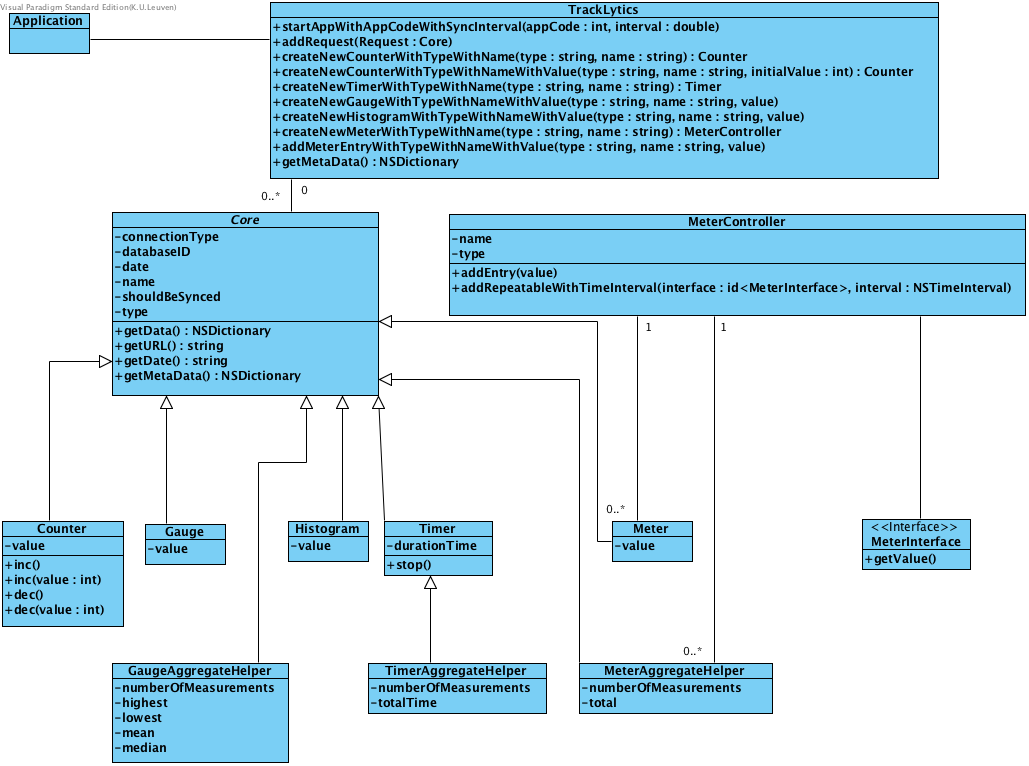
\includegraphics[scale=0.4]{Afbeeldingen/Implementatie/ClassDiagram}
  \caption{Klassediagram Tracklytics library.}
  \label{fig:fig}
\end{figure}
\section{Details Implementatie}
In deze sectie wordt er besproken welke technologie\"en er gebruikt zijn bij het ontwikkelen van de Tracklytics library.

\subsection{iOS Library}
De Tracklytics library beschreven in deze thesis werd ontwikkeld voor het iOS besturingssysteem. Voor het iOS besturingssysteem bestaan er twee programmeertalen om een applicatie, of in dit geval een library, te ontwikkelen, namelijk: Swift\cite{Swift} en Objective-C \cite{ObjectiveC}. Swift is een redelijk recente taal, op het moment van schrijven is deze nog geen twee jaar oud. De beide talen hebben evenveel functionaliteit, enkel de syntax verschilt hierbij en de prestaties van de taal. De mobile developer community biedt de meeste ondersteuning in Objective-C \cite{SwiftVSObjectiveC}. Dit vormt de hoofdreden dat er voor Objective-C gekozen is bij het ontwikkelen van de Tracklytics library.


\subsection{Klassediagram}
Het klassediagram duidt de klasses aan waaruit de Tracklytics library bestaat. De verantwoordelijkheden van de verschillende klasses worden uitgelegd in de volgende secties.

\subsubsection{TrackLytics}
De Tracklytics klasse stelt de klasse voor die de synchronisatie met de server verzorgt. De klasse is ook verantwoordelijk voor het creëren en het eventueel opslaan van de meetobjecten. De methodes van de Tracklytics library die gebruikt kunnen worden zijn statische methodes. De keuze hiervoor werd gebaseerd op twee redenen.

De Tracklytics library klasse die de methodes aanbiedt is geen objectgerichte klasse. Indien er een object van deze klasse zou gemaakt worden, zou deze elke keer na creatie bijna onmiddelijk niet meer gebruikt worden. Deze creatie van het object zorgt voor een overhead, dewelke wordt weggewerkt door het statisch maken van alle methodes die bruikbaar zijn door de developers. 

Een tweede reden kan men zien als de gebruiksvriendelijkheid. Men hoeft niet steeds opnieuw een Tracklytics object aan te maken om te kunnen monitoren. Het cre\"eren van een meetpunt kan hierdoor op \'e\'en lijn code gebeuren.\\


De Tracklytics klasse haalt de informatie over de applicatie uit de back end op aan de hand van de appCode die meegegeven moet worden bij het opstarten van de applicatie.

\subsubsection{Core}
Om de gemeenschappelijke elementen (de metadata) die er zijn per meting te combineren werd ervoor gekozen om die gemeenschappelijke elementen in een abstracte superklasse te steken. De gemeenschappelijke methodes worden ook in de Core klasse gestoken, zodat de subklasses indien nodig dit kunnen overriden. 

\subsubsection{Counter}
De counter klasse stelt een telobject voor. Je kan bij een counter een getal optellen en aftrekken. De inc() functie verhoogt de waarde van de counter met 1 terwijl inc(x) de waarde van de counter verhoogt met x. Hetzelfde geldt voor dec dat de waarde van de counter gaat verlagen. 

\subsubsection{Gauge}
De gauge klasse stelt een object met \'e\'en enkele waarde voor. Dit object wordt aangemaakt en eventueel opgeslagen met die waarde en gesynchroniseerd naar de server. 

\subsubsection{Histogram}
De gauge klasse en het histogram zijn maar op 1 punt verschillend en dat is in de back end. De waarde van het histogram wordt ergens anders opgeslagen dan de waarde van de gauge. In de Tracklytics library hebben ze dezelfde functionaliteit, enkel de URL naar waar de data verstuurd wordt verschilt. Dit zorgt ervoor dat in de back end de data op een andere plaats opgeslagen wordt en het dashboard zo deze data kan onderscheiden.

\subsubsection{Timer}
De timer klasse kan gebruikt worden om de lengte (in tijd) van een gebeurtenis te meten. Bij het aanmaken van de timer wordt de huidige timestamp bijgehouden. De stop() methode neemt de huidige timestamp en vergelijkt die met degene die werd bijgehouden. Dit resultaat stelt de duur van het evenement voor. Indien de programmeur de methode stop() nooit aanroept, wordt de timer niet gesynchroniseerd naar de server zodat er geen foute data tussen de data in de database staat. 

\subsubsection{Meter}
Een meter werd ontwikkeld om een reeks van waarden te kunnen meten. Om dit voor de developer makkelijk te maken zijn er  3 componenten uitgedacht: de \texttt{Meter}, de \texttt{MeterController} en de \texttt{MeterInterface}. De meter component vormt een uitzondering als er gekeken wordt naar het flow diagram uit de vorige sectie \ref{fig:flow2}. In plaats van dat een \texttt{Meter} object wordt terug gegeven, wordt er een \texttt{MeterController} object terug gegeven. Een \texttt{MeterController} beheert het collecteren van de data. 

\paragraph{Meter}
Het meter object stelt het object voor  dat opgeslagen wordt en dat gesynchroniseerd wordt naar de server. Het object houdt de waarde bij en ook het tijdstip van aanmaken. Per meting dat de meter in de applicatie doet, moet er een \texttt{Meter} object aangemaakt worden. Dit is een van de reden dat de \texttt{MeterController} bestaat. 

\paragraph{MeterController}
De metercontroller zorgt ervoor dat nieuwe meters aangemaakt kunnen worden. De metercontroller bevat de naam en het type van de meter. De keuze om de meters op deze manier aan te maken berust zich op het feit dat zo niet telkens opnieuw het type van de meter moet meegegeven worden, omdat de metercontroller dit al doet en ook om de data periodiek op te kunnen halen. De metercontroller biedt een mogelijkheid aan om via de MeterInterface\ref{Klassediagram:MeterInferface} periodiek een waarde op te halen. Deze functionaliteit zorgt ervoor dat de developer niet telkens na een bepaald interval zelf de metercontroller aan moet roepen, maar dat dit automatisch gebeurt.

\paragraph{MeterInterface}\label{Klassediagram:MeterInferface}
De meterinterface wordt gebruikt om automatisch een waarde op te halen. De metercontroller roept de enige methode die deze interface aanbiedt (\texttt{getValue()}) aan elke keer een gegeven tijdsinterval voorbij is. De developer moet deze methode implementeren in de klasse waar deze data gecollecteerd moet worden.  



\subsubsection{Aggregatie}
Zoals besproken in de architectuur \ref{Arch:Aggregatie} vormt \'e\'en van de uitbreidingen van de monitoring library de developer de keuze te geven tussen het aggregeren van de data in de back end of op het toestel van de gebruiker zelf. Om deze uitbreiding te ondersteunen werd ervoor gekozen om voor drie types meetobjecten de mogelijkheid tot aggregatie toe te voegen aan de Tracklytics library, namelijk: \texttt{Gauge, Meter en Timer}. De \texttt{Counter en Histogram} worden niet geaggregeerd, omdat er normaal gezien maar per type \'e\'en counter bestaat en omdat een histogram alle waardes nodig heeft om een model op te stellen. Er bestaat geen verschil tussen de code die de developer moet implementeren in de applicatie om van deze functionaliteit gebruik te kunnen maken.\\

\paragraph{De GaugeAggregateHelper} stelt de klasse voor die de waarden van de \texttt{Gauges} verwerkt op het toestel. In plaats van dat er telkens een nieuwe \texttt{Gauge} aangemaakt wordt, worden de volgende waarden berekend: \textit{hoogste waarde, laagste waarde, gemiddelde en mediaan}. Het totaal aantal metingen wordt telkens met \'e\'en verhoogd. Deze functionaliteit werd ge\"implementeerd in de Tracklytics klasse bij de \texttt{createNewGauge} methode. 

\paragraph{De MeterAggregateHelper} collecteert de waardes die in een \texttt{Meter} object zouden geplaatst worden. In plaats van het aanmaken van een nieuwe \texttt{Meter} wordt het totaal verhoogd met de gemeten waarde en wordt het totaal aantal metingen met \'e\'en verhoogd. Dit heeft zeker geen invloed op de code die de developer moet schrijven, omdat de \texttt{MeterController} het aanmaken van de \texttt{Meters} verzorgt.

\paragraph{De TimerAggregateHelper} klasse is iets complexer. De developer moet een Timer object terug krijgen om de \textit{stop} methode te kunnen aanroepen. Dit stelt de reden voor dat de TimerAggregateHelper als superklasse de Timer heeft. Zo moet de developer zijn code niet aanpassen om deze functionaliteit te gebruiken. De Tracklytics klasse zorgt bij het aanroepen van de \textit{createTimer} methode dat de huidige tijd wordt gezet in de TimerAggregateHelper. Indien de \textit{stop} methode wordt aangeroepen, dan berekent de TimerAggregateHelper de verstreken tijd, telt deze op bij de totale tijd en verhoogt het totaal aantal metingen met \'e\'en.



\subsection{Back end}
De data die de Tracklytics library doorstuurt vanaf het toestel van de gebruiker moet opgeslagen worden in een database. Zo kan deze data later verwerkt worden en worden weergegeven in het dashboard. Er moet een keuze gemaakt worden over het besturingssysteem, de database en de programmeertaal van de back end.\\

De server draait in OpenStack, een cloud platform. Deze werd gedeployed als infrastructure-as-a-service (IaaS). Dit wil zeggen dat dit meerdere virtuele servers kan aanbieden (zelfs meerdere virtuele servers als fysieke servers). Dit biedt een abstractie en schermt de virtuele server af van andere virtuele servers. Een gebruiker kan zelf nieuwe virtuele servers aanmaken. Elke virtuele server heeft zijn eigen besturingssysteem, te kiezen uit een lijst van images aangeboden door OpenStack\cite{OpenStack}.

In de Tracklytics architectuur werd gekozen voor een Linux distributie (in dit geval Ubuntu \cite{Ubuntu}). Deze keuze werd gemaakt op basis van de gebruiksvriendelijkheid van dit besturingssysteem. Zo is het gemakkelijk om een web server op te zetten en een database te installeren. Er werd voor Ubuntu gekozen, omdat dit de meest gekende en meest gebruikte Linux distributie is. \\

In de database wordt alle data opgeslagen, dat wil zeggen dat dit een van de meest belangrijke onderdelen van de Tracklytics architectuur vormt. De metadata die gecollecteerd wordt per applicatie is in vele gevallen hetzelfde. De parameters die verschillen zijn: het type toestel, het type internet connectie en de versie van de applicatie. Dit gegeven zorgt ervoor dat de metadata vaak hetzelfde is. Indien de metadata uit de data komende van de Tracklytics library wordt uitgehaald kan er relatief veel opslagruimte gespaard worden, omdat deze metadata niet in elke entry in de database aanwezig moet zijn, enkel een verwijzing naar waar die metadata staat. Er werd voor gekozen om een relationele database te kiezen, namelijk MySQL \cite{MySQL}. De gebruikte tabellen zijn met behulp van SQL queries gecombineerd in views om de data overzichtelijk te maken. \\

De back end heeft in de Tracklytics library twee functies, namelijk: het verwerken en opslaan van de data in de database en het opvragen van data uit de database om het dashboard van de data te voorzien. De keuze is gevallen op PHP \cite{PHP} als programmeertaal. Met PHP is het eenvoudig om een database connectie op te zetten en via SQL queries deze data in of uit de database te krijgen. Een tweede voordeel van PHP is dat deze met POST data om kan. Op deze manier kan de data in de request van de Tracklytics library verborgen worden in de request en moet deze niet rechtstreeks doorgegeven worden in bijvoorbeeld de URL zelf. Zo bestaat er meer veiligheid en privacy van de data. \\

\subsection{Structuur database}
\begin{figure}[!h]
  \centering
  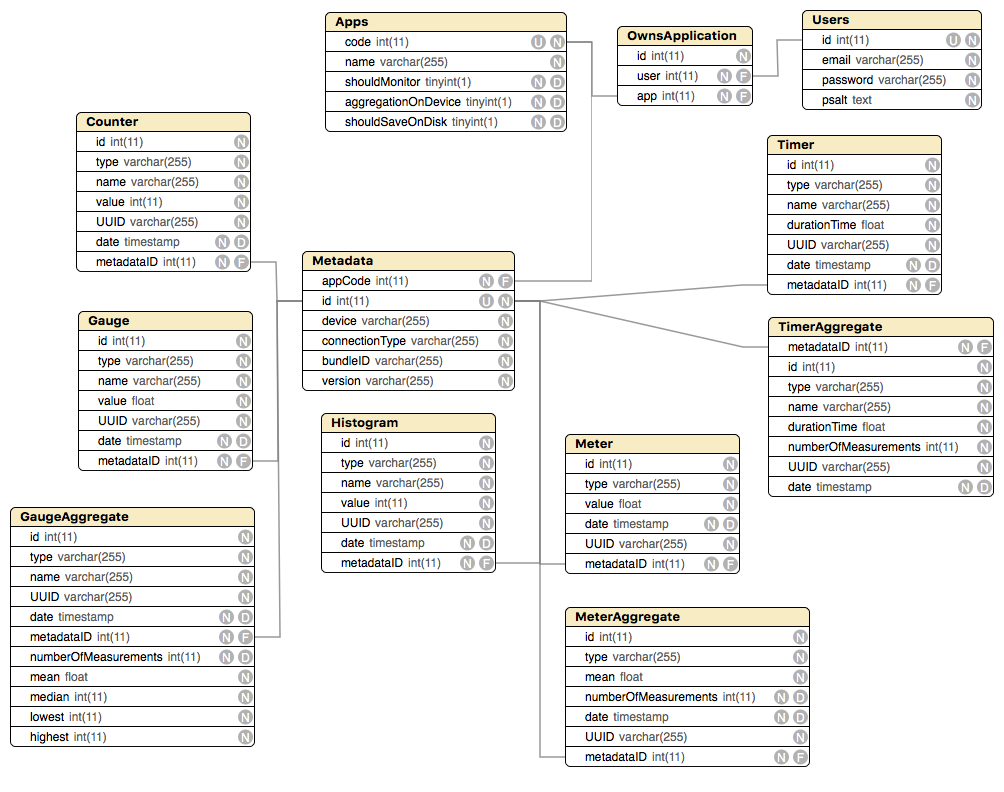
\includegraphics[scale=0.4]{Afbeeldingen/Implementatie/DatabaseDiagram}
  \caption{Structuur van de Tracklytics database.}
  \label{fig:database}
\end{figure}

In bovenstaande figuur \ref{fig:database} wordt de structuur van de Tracklytics library getoond. Voor elk type meetobject werd er een tabel aangemaakt waarin de gegevens opgeslagen worden. Voor elk type geaggregeerd object werd er een aparte tabel aangemaakt omdat deze een andere structuur nodig hebben dan de originele objecten. De metadata wordt opgeslagen in een aparte tabel en vanuit elk type meetobject wordt hier naar gelinkt met behulp van de metadataID. Elke applicatie die de Tracklytics library gebruikt, heeft een entry in de Apps tabel om deze applicatie te identificeren. De OwnsApplication en User tabel worden gebruikt door het dashboard om de developers die het dashboard gebruiken te linken aan de applicaties die ze geregistreerd hebben. \\

\paragraph{De Metadata} tabel bevat per applicatie de metadata die gelinkt wordt aan de entries in een tabel van de meetobjecten. Hierin worden de volgende eigenschappen gebundeld: een link naar de applicatie waar deze entry bij hoort, het type toestel, welke soort netwerkverbinding de gebruiker had, de versie van de applicatie en het bundleID van de applicatie, wat een identificatie van die bepaalde applicatie voorstelt vanuit het iOS systeem. Deze tabel verkleint de tabellen van de meetobjecten, omdat er enkel een link naar een entry in deze tabel moet staan en niet alle metadata bij in de tabel van het meetobject moet staan. 

\paragraph{De tabellen van de meetobjecten} bevatten de data die door de library gecollecteerd zijn. Zoals hierboven vermeld hebben de entries in de tabel een link naar een entry in de metadata tabel. De meetobjecten en de metadata worden gecombineerd in een view per type meetobject om zo per meting te kunnen zien welke metadata de meting heeft. Dit is eenvoudiger voor het ophalen van de data voor het dashboard.

\subsection{Structuur back end}
De back end werd opgedeeld in twee delen, namelijk een deel waarmee de mobiele library in contact staat en een deel waarmee het dashboard in contact staat. Het doel van het eerste deel is om de data die van de mobiele library komt te verwerken en op te slaan in de database. Het doel van het tweede deel is om de gegevens uit de database op te halen en door te geven aan het dashboard. Om de data die van de mobiele library komt op te slaan in de database werd ervoor gekozen om per type meetobject een apart PHP bestand aan te maken die de data van dat type meting verwerkt en opslaat in de database. Het dashboard haalt de data die hij nodig heeft op via specifieke PHP bestanden ontwikkeld om het dashboard van data te voorzien, zoals bijvoorbeeld het totaal aantal counts. 




\subsection{Dashboard}\label{visualisatie}
Het Tracklytics dashboard werd ontworpen om de gegevens van de applicatie in grafieken en details weer te geven om hieruit een conclusie te kunnen trekken over het functioneren van de applicatie. Het dashboard werd ontworpen als webapplicatie in plaats van een desktop applicatie. De voordelen hiervan zijn: software updates worden automatisch doorgevoerd zonder dat er tussenkomst van de gebruiker nodig is, het is cross platform, omdat het in de browser draait en er is geen installatie vereist. \\

Om de webapplicatie te ontwikkelen werd er gebruik gemaakt van AngularJS \cite{AngularJS}. De reden hiervoor is dat dit een zeer handig framework is voor het ontwikkelen van dynamische websites. Dit framework bindt stukken HTML code aan JavaScript code, wat ervoor zorgt dat het DOM gemakkelijk manipuleerbaar is door JavaScript.
Met AngularJS is het eenvoudig om grafieken en gegevens die getoond moeten worden meermaals te herhalen met andere gegevens in. Zo kunnen de verschillende grafieken onder elkaar geplaatst worden zonder telkens de HTML code in JavaScript aan te moeten passen. Een bijkomstig voordeel is dat de data in de verschillende tabbladen maar eenmalig ingeladen moet worden, omdat AngularJS ervoor zorgt dat als je op een tab drukt niet de hele webpagina opnieuw wordt ingeladen, maar enkel de view die verandert ingeladen wordt.

Om de grafieken weer te kunnen geven, werd ervoor gekozen om Chart.js\cite{ChartJS} (voor AngularJS) te gebruiken. Dit framework neemt data die in AngularJS variabelen gezet worden en geeft deze weer in een gekozen grafiek (bv.~ lijn-grafiek of staafdiagram). Chart.js is een simpele manier om snel een grafiek weer te kunnen geven, het werkt out-of-the-box en er zijn een aantal zeer handige opties die kunnen aangepast worden. 

Om de histogrammen en de meters bruikbaarder te maken, werden hier sliders (\ref{fig:DasbhoardHistogram}, \ref{fig:DasbhoardMeter}) bij toegevoegd om bij de histogrammen het interval te veranderen en zo een kleinere dataset te gebruiken. Bij de meters kan de dataset verkleind worden door het tijdsinterval te wijzigen. Een slider boven de grafieken zorgt ervoor dat de dataset verkleind kan worden. Deze slider werd ge\"implementeerd met behulp van de AngularJS-slider \cite{AngularSlider}.\\


De grafieken worden per soort meetobject weergegeven, er bestaat dus een aparte pagina voor de counters, de gauges, de timers, de meters en de histogrammen. Zo heeft een developer een overzicht per type meting. De grafieken die weergegeven worden zijn basisgrafieken, deze zijn enkel opgedeeld door de namen die aan de metingen gegeven zijn. De developer kan hier enkel basisinformatie uithalen. Om een dieper detailniveau te verkrijgen werd ervoor gekozen om per grafiek een gedetailleerdere pagina weer te geven. De grafiek wordt dan opgesplitst door verschillende eigenschappen te gebruiken. De volgende eigenschappen worden gebruikt om de grafieken op te delen: het type toestel, de versie van de applicatie en het type connectie. Deze worden onderling nog gecombineerd om nog extra in detail de gemeten data te kunnen bekijken. Aan de hand hiervan kunnen developers een concreet overzicht krijgen over de prestaties en het gebruik van de applicatie. \\

\paragraph{De counters \ref{fig:DasbhoardCounter}} worden weergegeven in een staafdiagram, zodat er snel gezien kan worden welke counter het meeste tellingen heeft. In de detailpagina wordt er opgesplitst per toestel en per versie en deze worden met elkaar gecombineerd. Zo kan de developer een beter overzicht krijgen naar de tellingen.\\

\paragraph{De timers \ref{fig:DasbhoardTimer}} worden als gemiddelde weergegeven, niet in een grafiek maar als tekst. Zo kan de developer snel kijken wat de gemiddelde duur is. In de detailpagina worden deze metingen opgesplitst op welke internetverbinding het toestel had, welk toestel het was waarop gemeten werd en welke versie. Deze worden onderling gecombineerd om een gedetailleerder beeld te geven aan de developers.\\

\paragraph{De gauges \ref{fig:DasbhoardGauge}} worden weergegeven als de gemiddelde waarde die gemeten werd. Zo wordt er een snel overzicht gegeven aan de developers. Developers kunnen deze data dieper bekijken op de detailpagina. Hier worden de volgende overzichten aangeboden: het gemiddelde, de mediaan, de laagste en de hoogste waarde. \\

\paragraph{De histogrammen \ref{fig:DasbhoardHistogram}} worden weergegeven als histogrammen, in een staafdiagram met daaronder de gegevens die belangrijk zijn over het histogram, namelijk: de mediaan, het gemiddelde, standaarddeviatie. Er zijn nog enkele andere gegevens bijgevoegd die belangrijk kunnen zijn, namelijk: het verschil tussen de grootste en de kleinste waarde, het percentage lager dan het gemiddelde en het percentage hoger dan het gemiddelde. In de detailpagina wordt het histogram opgedeeld op basis van het toestel en/of de versie om een gedetailleerder beeld te krijgen.
Er werd gekozen om een slider toe te voegen aan de histogrammen om het bereik te kunnen verkleinen. Er is de mogelijkheid om de maximum- en minimumwaarde aan te geven met behulp van deze slider. \\

\paragraph{De meters \ref{fig:DasbhoardMeter}} worden weergegeven als een lijngrafiek met daarop het gemiddelde per dag. Er werd een slider voorzien om de developer de kans te geven de dataset te verkleinen door het bereik aan te passen en zo aan te geven van welke dagen hij het overzicht wil zien. Indien de dataset minder dan drie data bevat werd er voor gekozen om de data per drie uren weer te geven, zodat er meer op detail in kan gegaan worden. In de detailpagina wordt deze data opgesplitst op basis van het type toestel en/of de versie waarop gemeten werd. \\ 


In het dashboard werd ruimte voorzien om instellingen van de applicatie op afstand te wijzigen \ref{fig:DasbhoardSettings}. De developer kan kiezen of de applicatie gemonitord moet worden, of dat de aggregatie op het toestel moet gebeuren of in de back end en hij kan kiezen of de data tijdelijk op de harde schijf opgeslagen moet worden of niet. Deze remote functies zorgen ervoor dat de developer niet telkens een nieuwe versie moet uitrollen om deze instellingen te wijzigen.\\


De data die nodig is om de titels en de gegevens voor de grafieken in te laden moet uit de back end gehaald worden. Deze werd, zoals in vorige sectie aangehaald, geschreven in PHP. \\ 

Er is enorm veel werk gekropen in het ontwikkelen van dit dashboard. Dit omdat het dashboard from scratch ontwikkeld is. De reden hiervoor is dat de bestaande dashboards, die vrij te gebruiken zijn, geen oplossing gaven voor de visualisatie die ik wou geven. Het ontwikkelen van het dashboard (inclusief het opzetten van alle achterliggende systemen zoals de database en dergelijke) in combinatie met het ontwikkelen en het tweaken van de library heeft meer dan 200 uur tijd in beslag genomen.

\begin{figure}[!h]
  \centering
  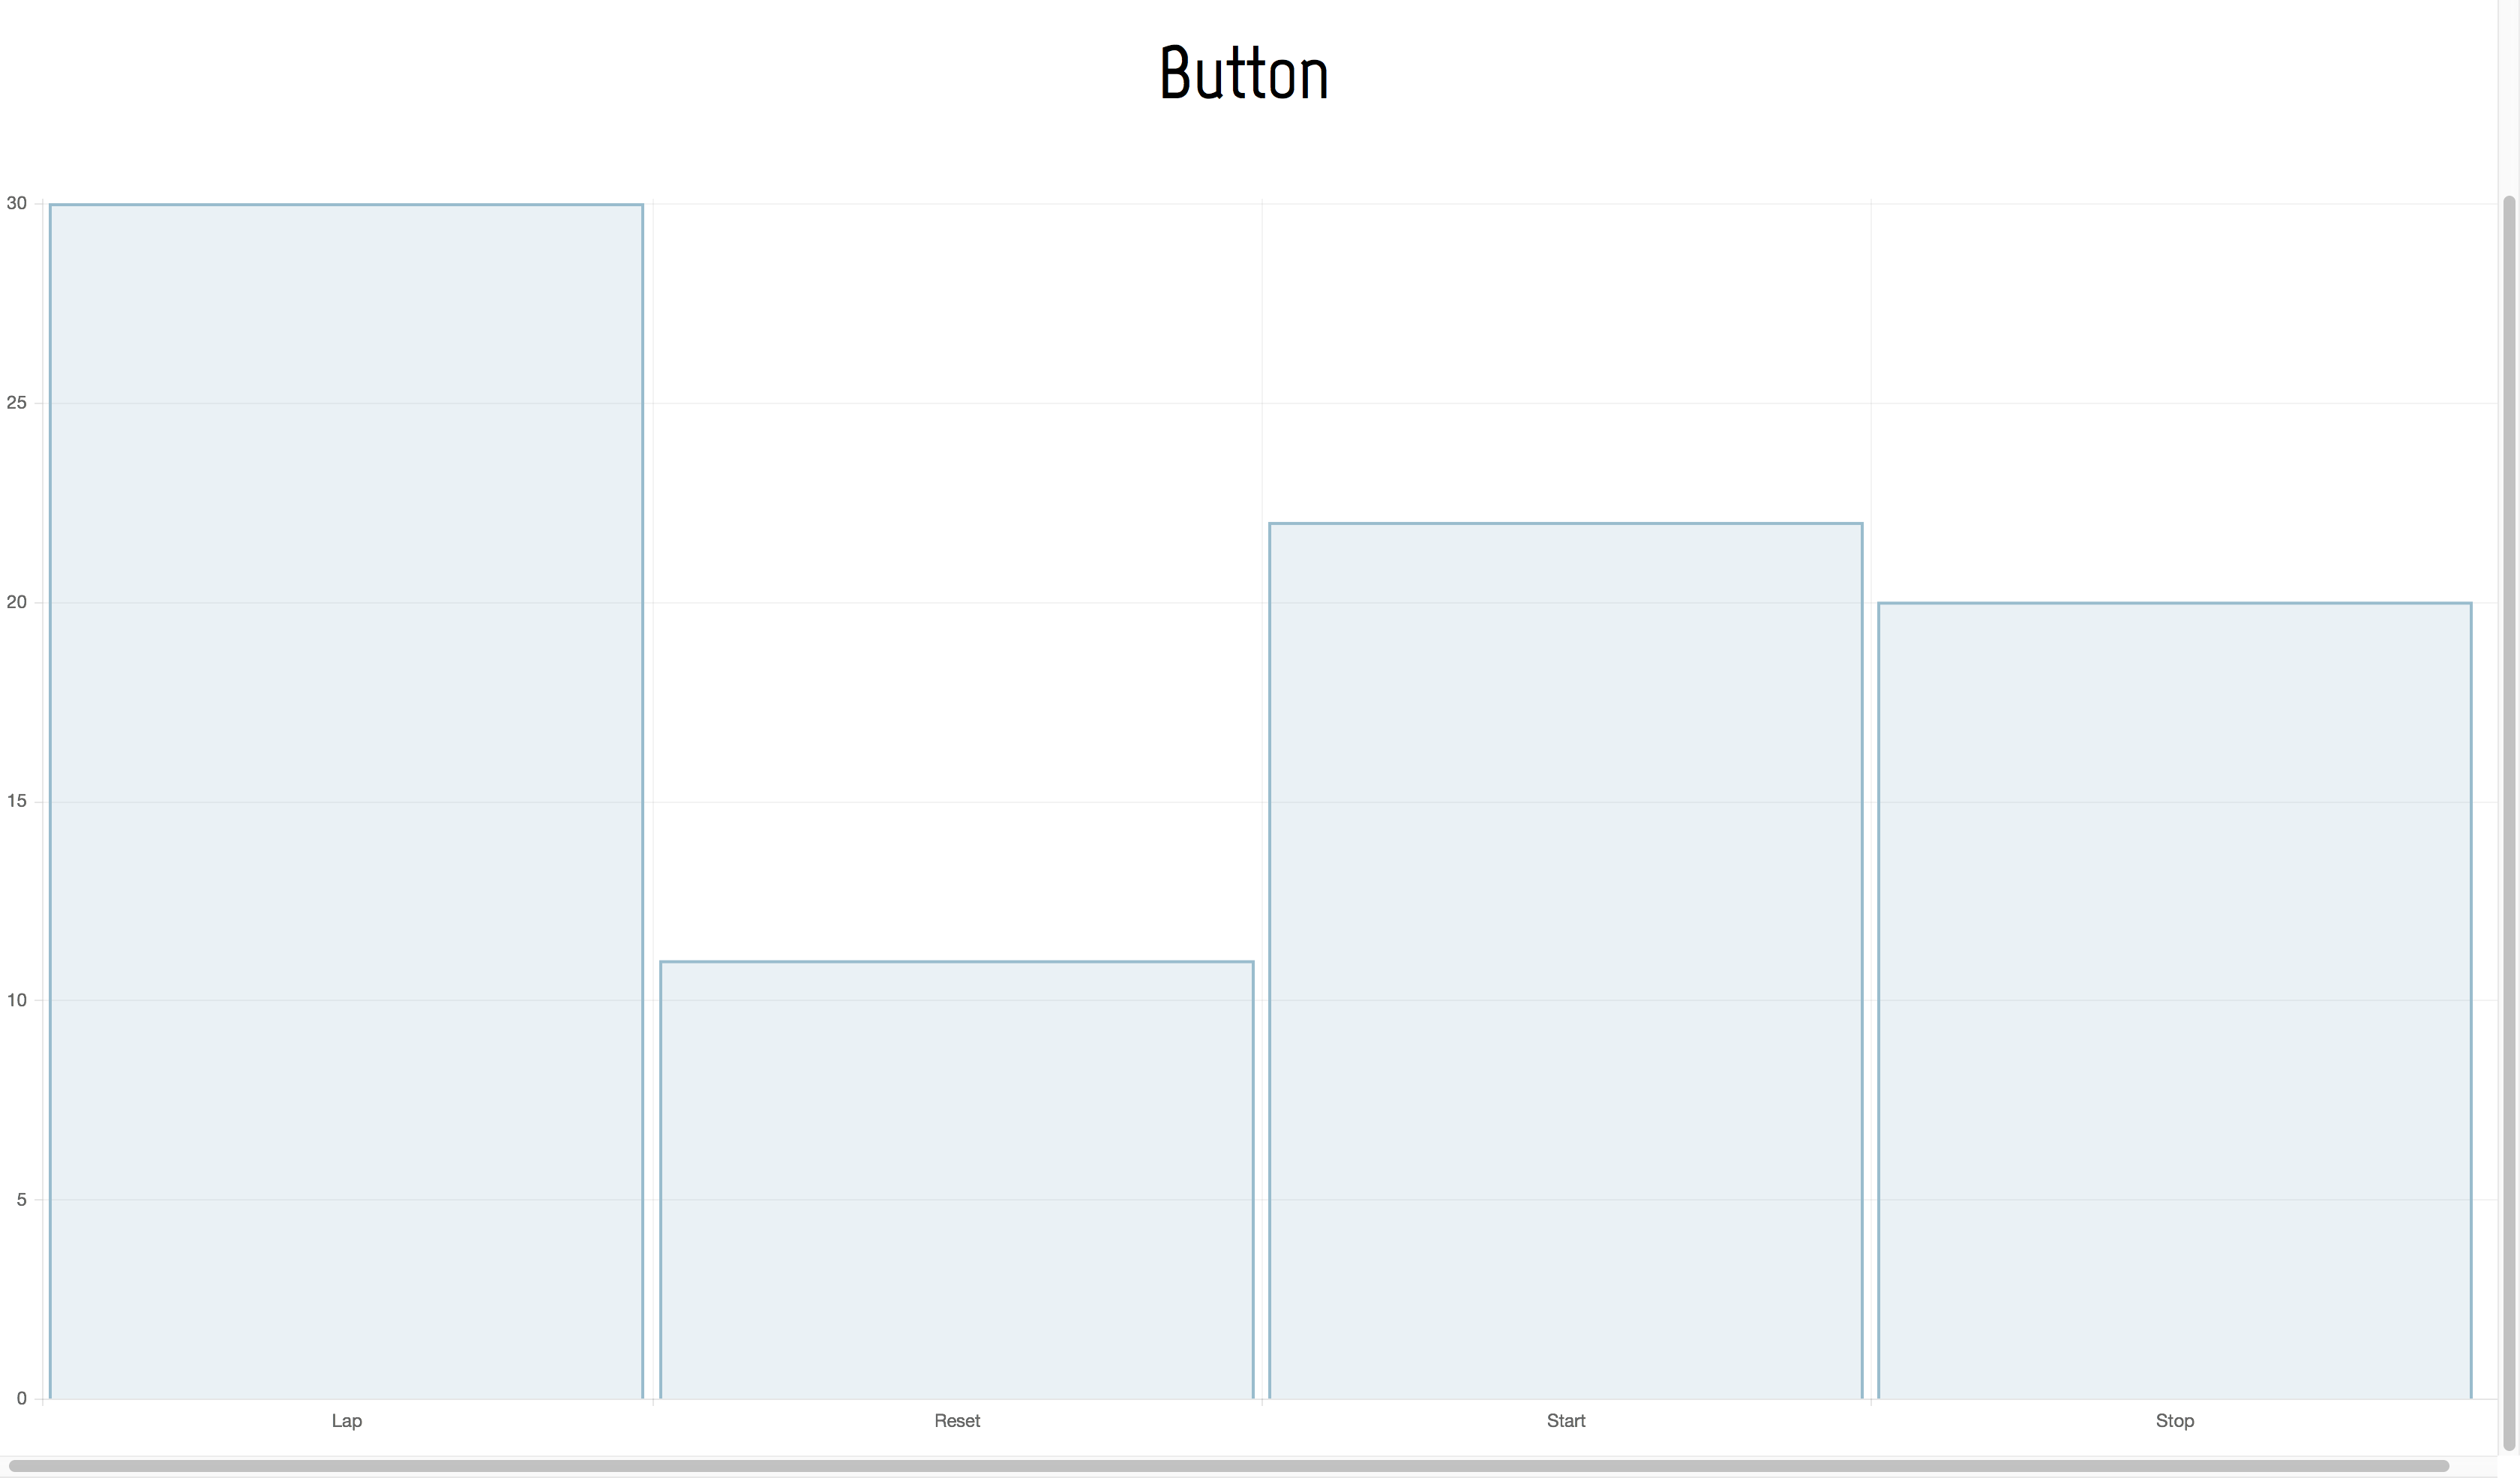
\includegraphics[scale=0.2]{Afbeeldingen/Implementatie/Counter}
  \caption{Dashboard: \texttt{Counter} overzicht.}
  \label{fig:DasbhoardCounter}
\end{figure}

\begin{figure}[!h]
  \centering
  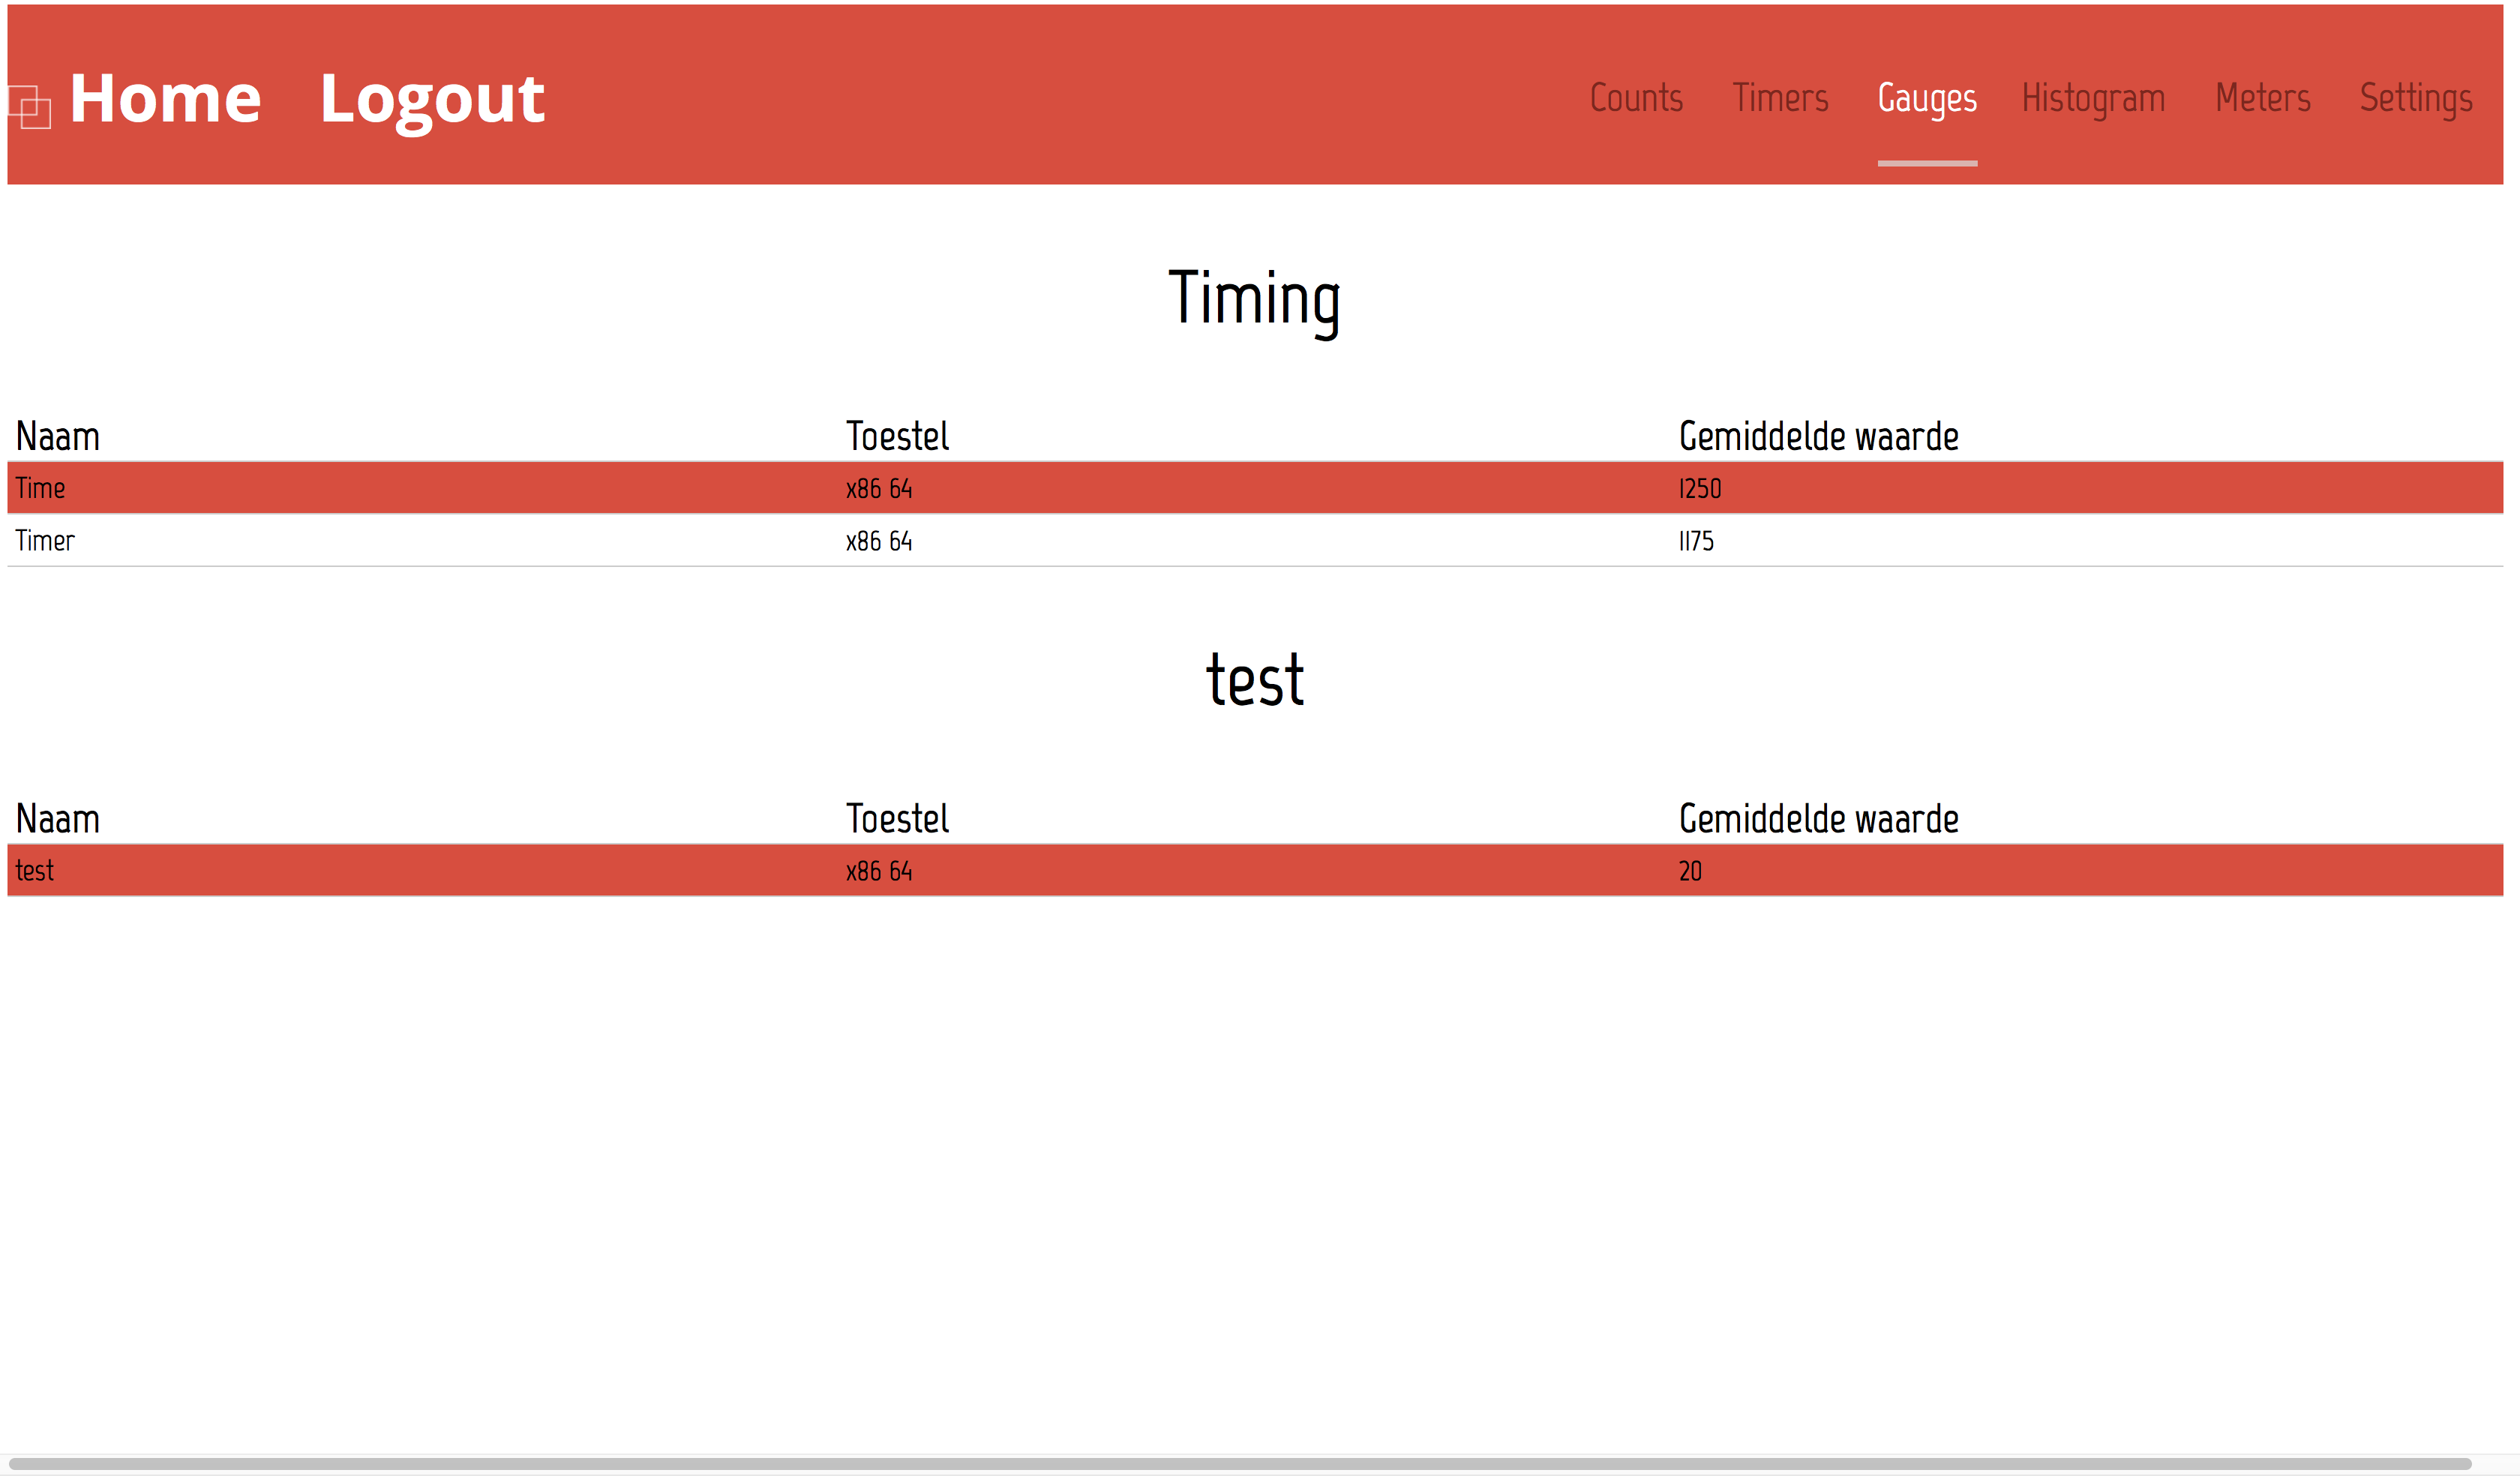
\includegraphics[scale=0.2]{Afbeeldingen/Implementatie/Gauge}
  \caption{Dashboard: \texttt{Gauge} overzicht.}
  \label{fig:DasbhoardGauge}
\end{figure}

\begin{figure}[!h]
  \centering
  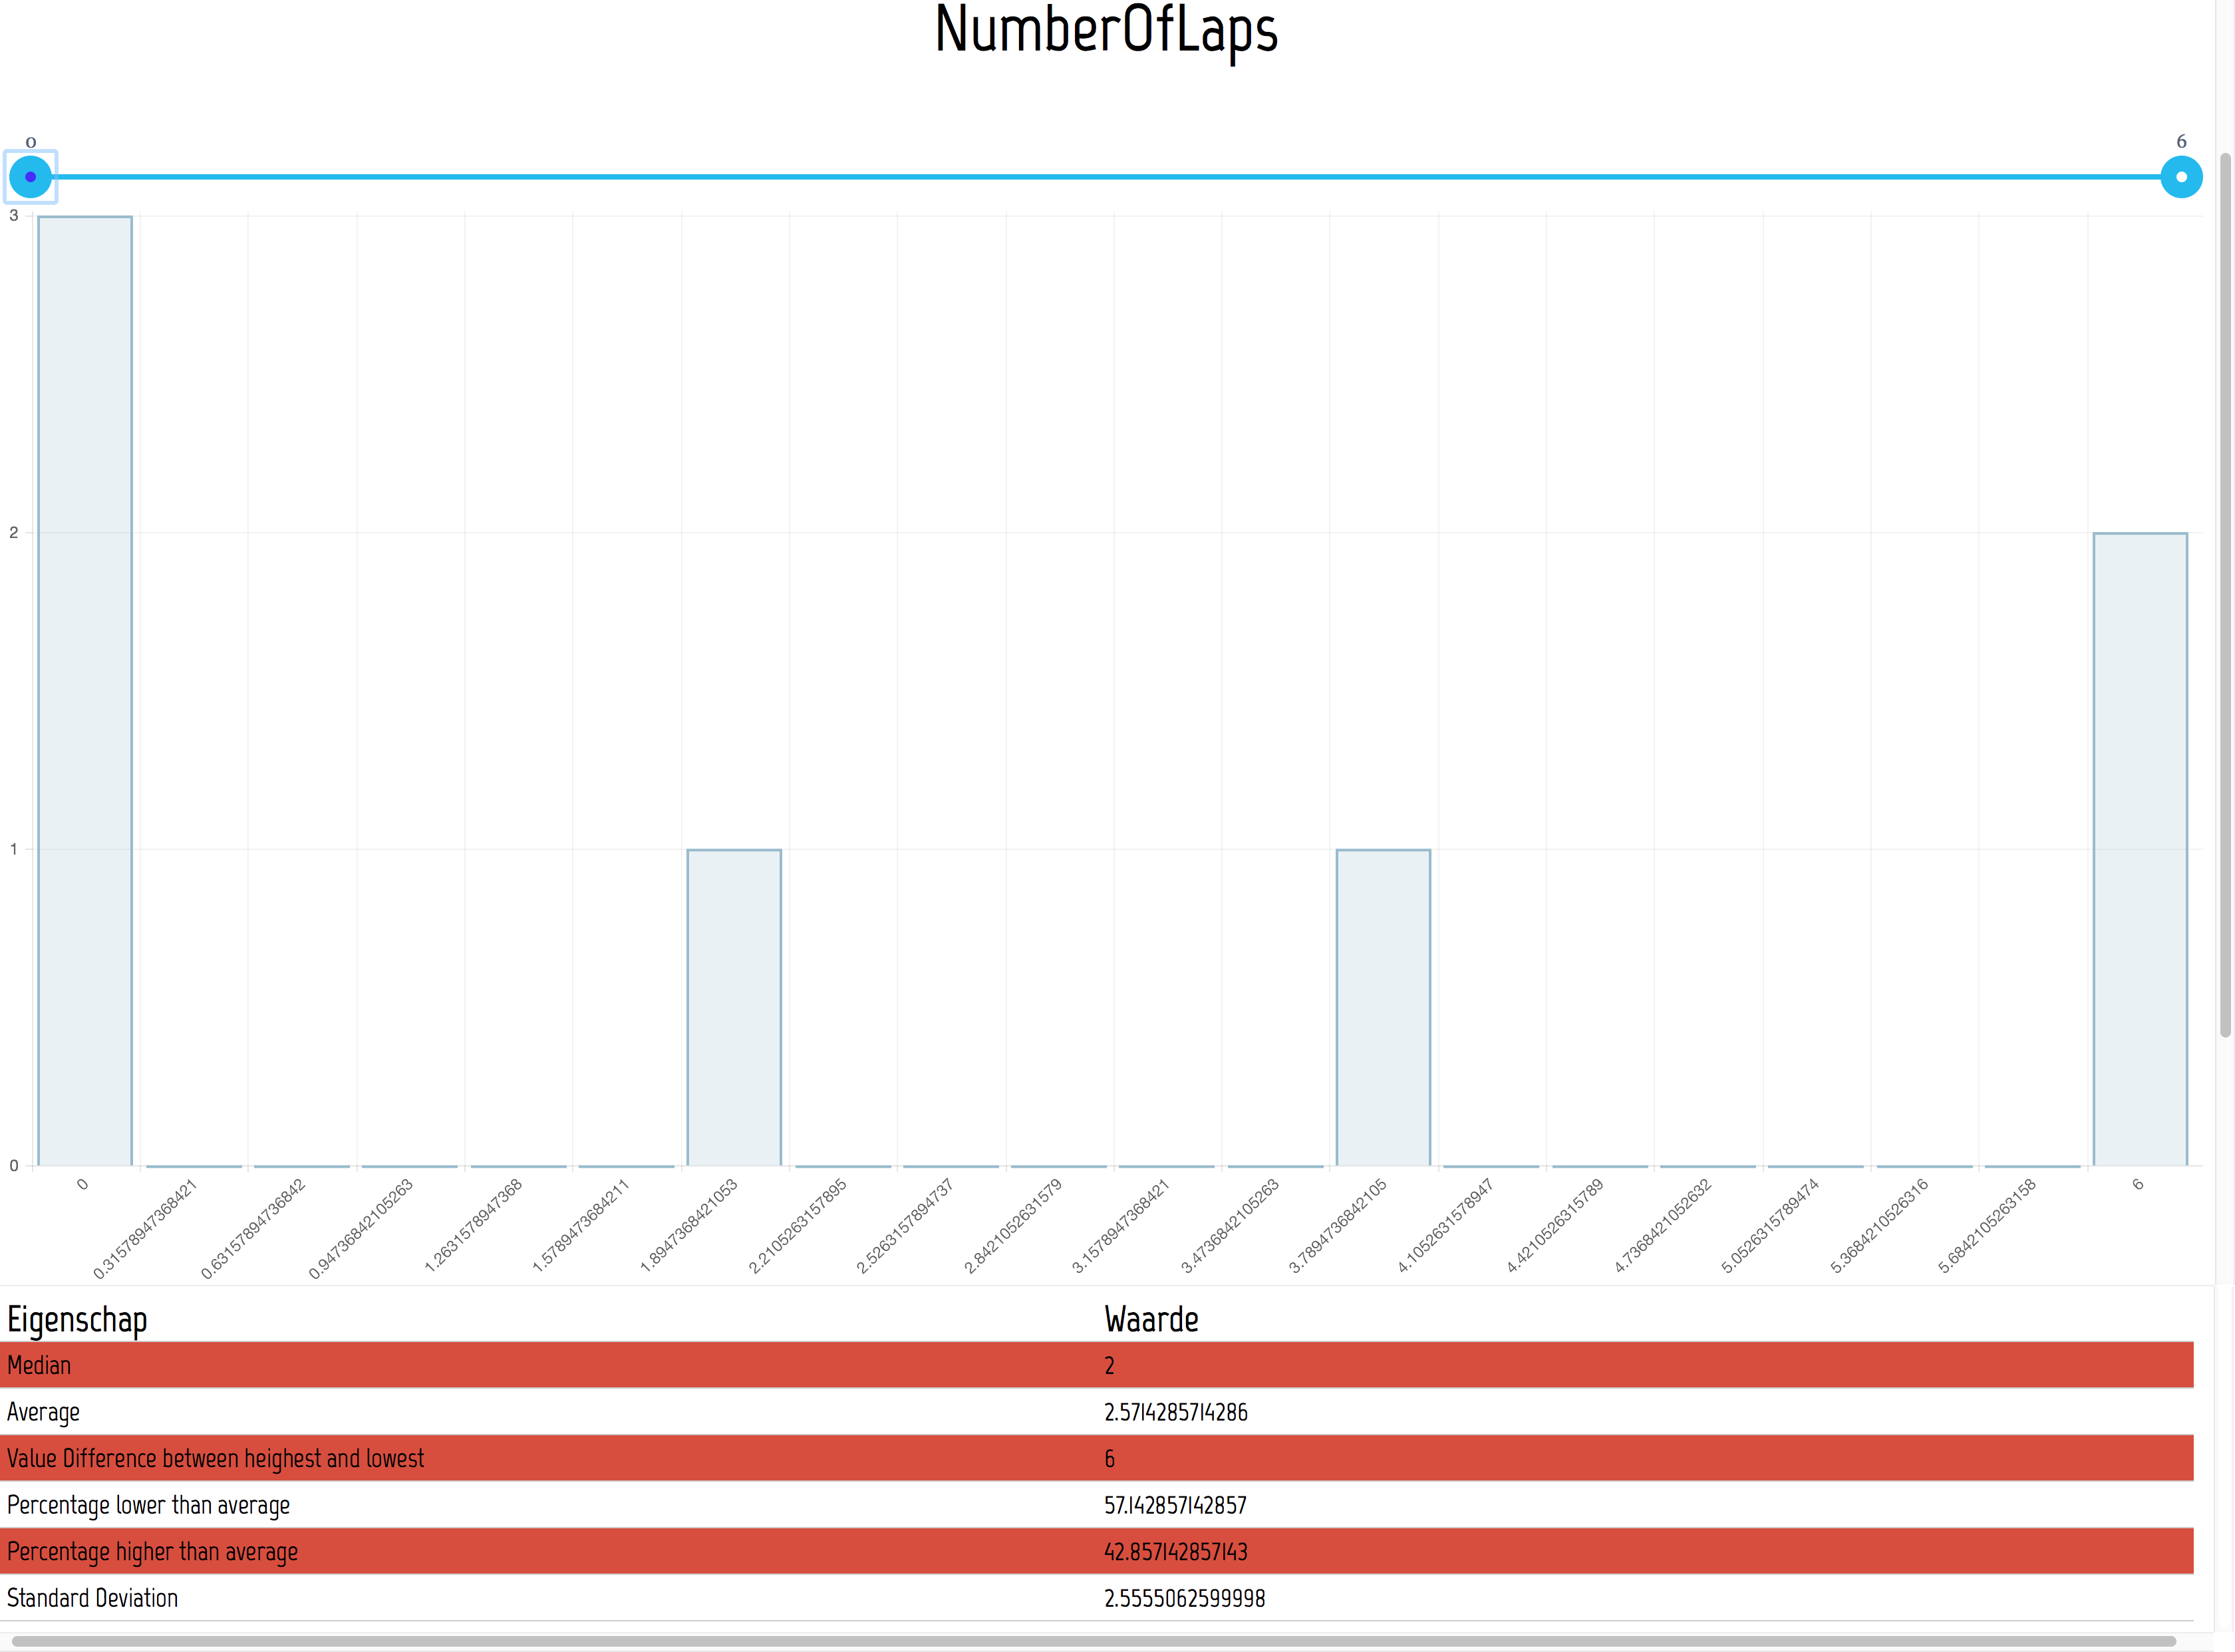
\includegraphics[scale=0.2]{Afbeeldingen/Implementatie/Histogram}
  \caption{Dashboard: \texttt{Histogram} overzicht.}
  \label{fig:DasbhoardHistogram}
\end{figure}

\begin{figure}[!h]
  \centering
  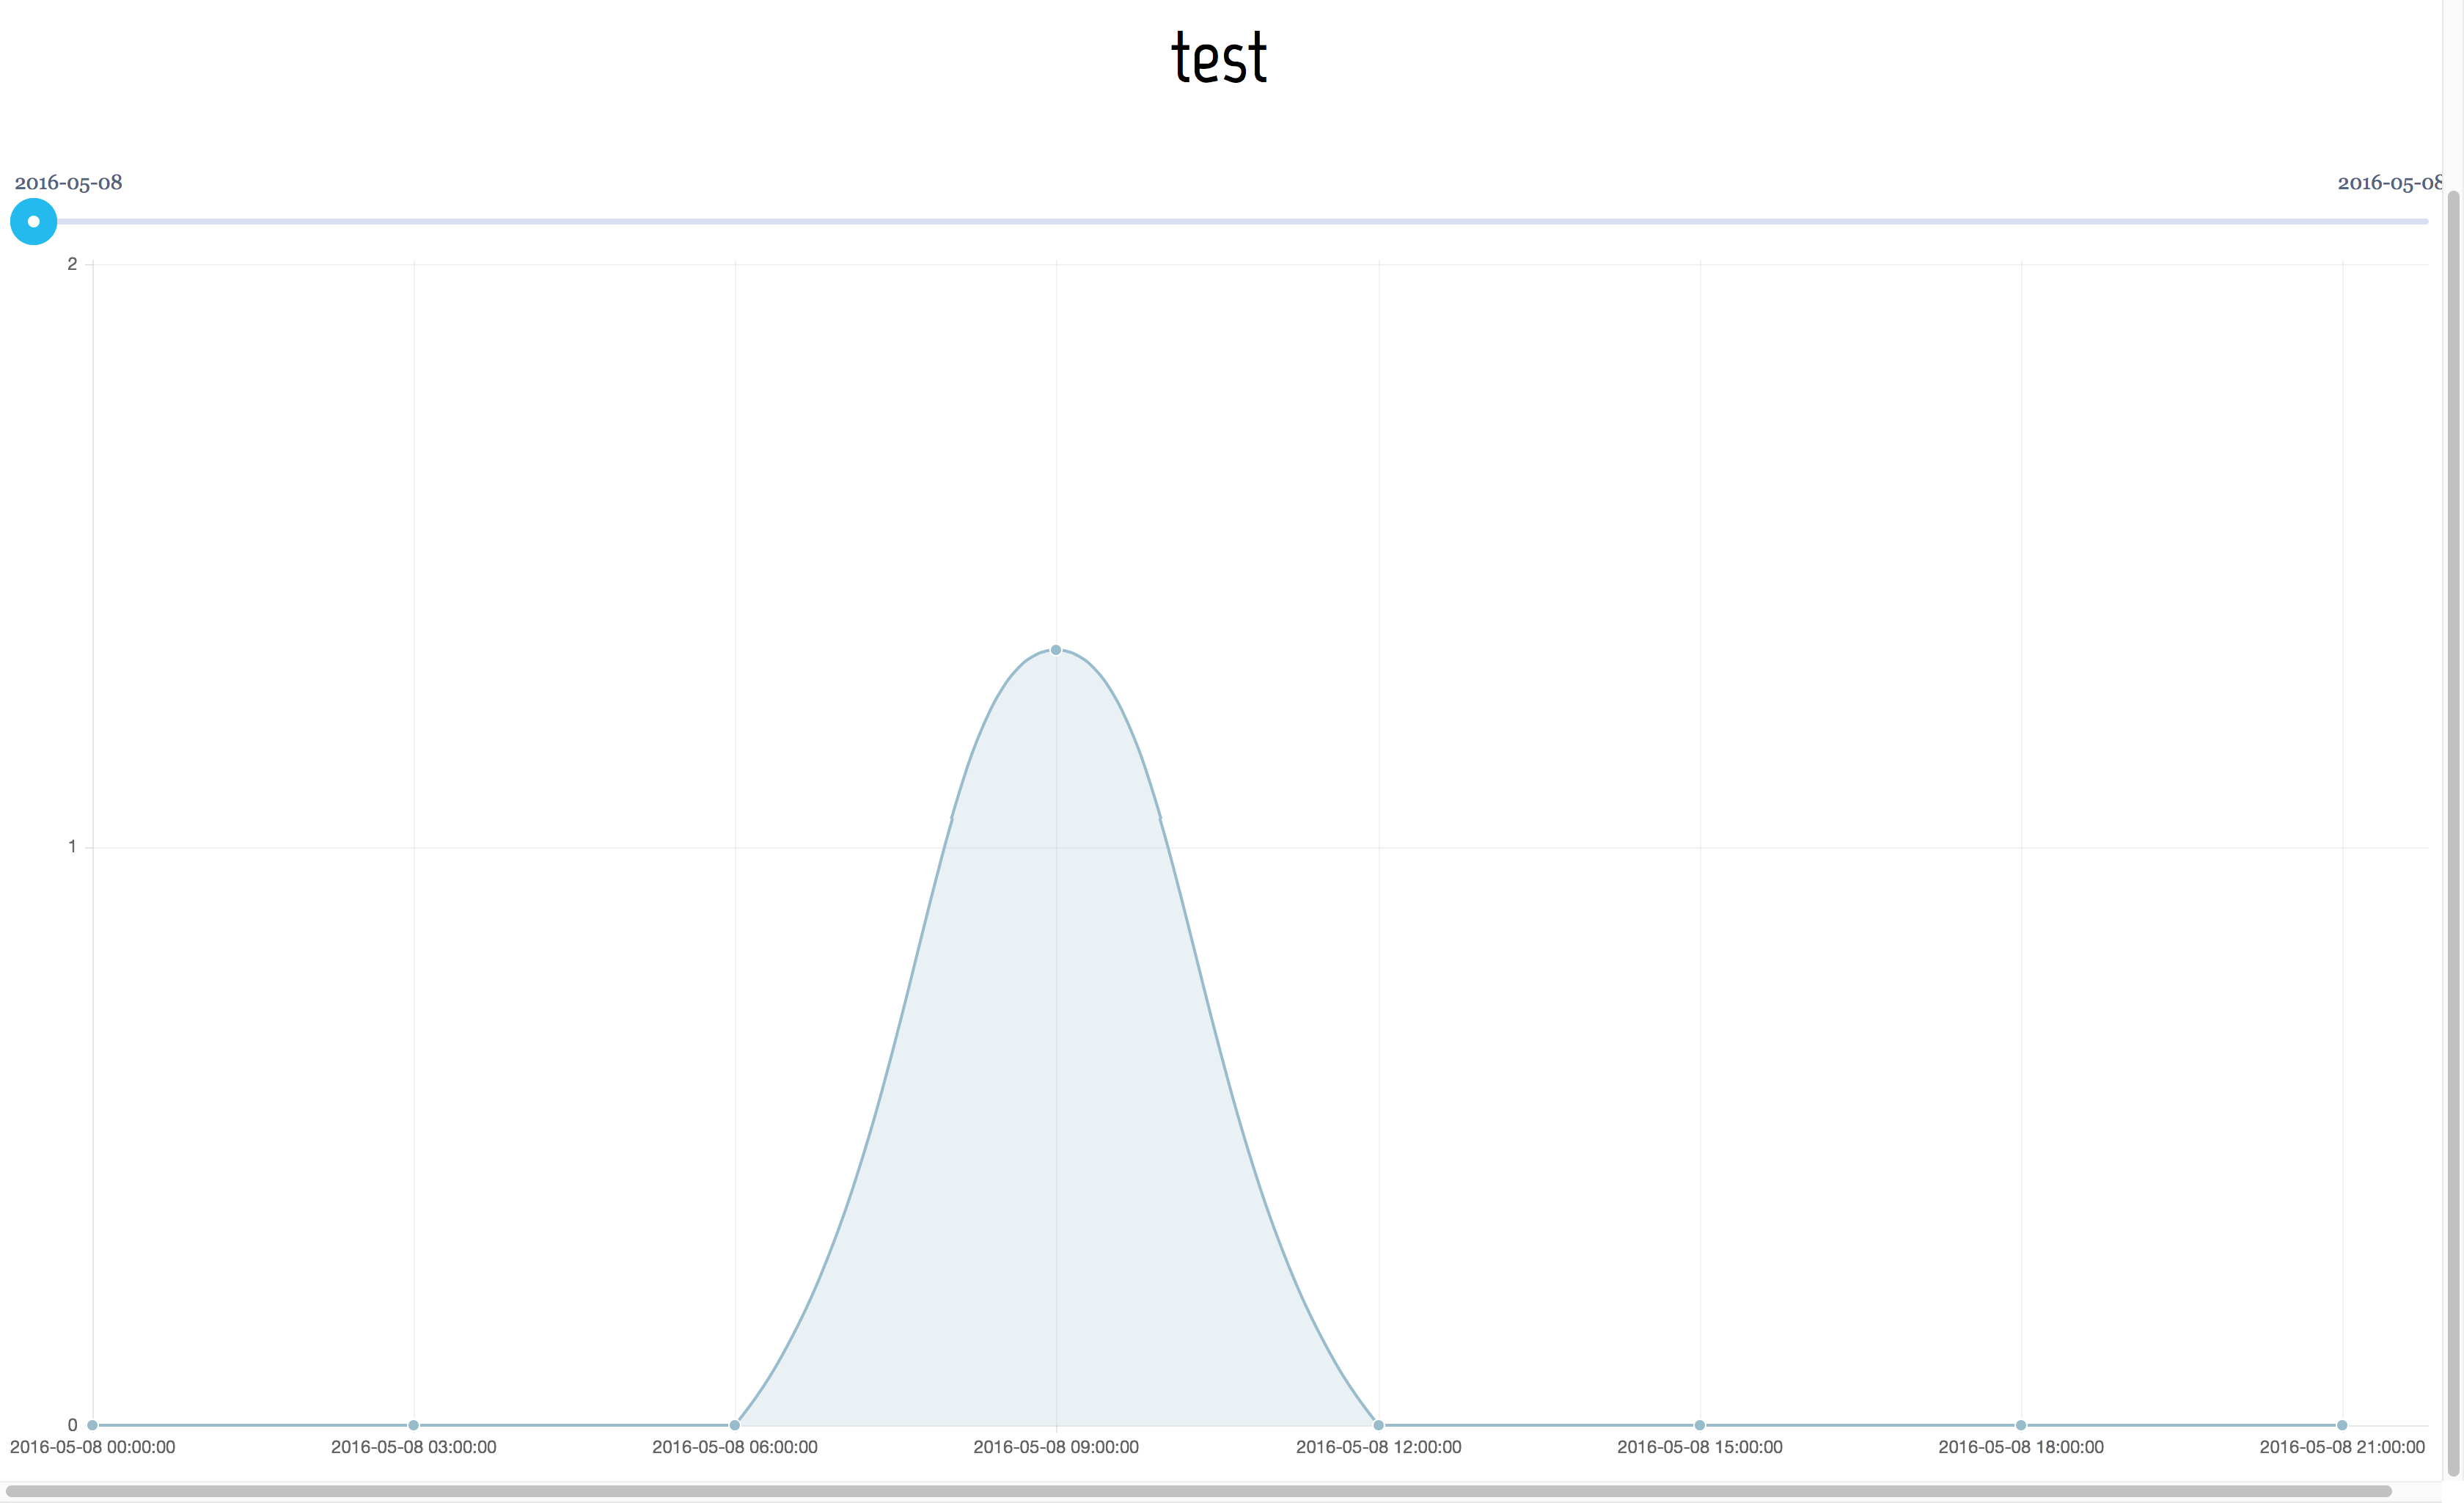
\includegraphics[scale=0.2]{Afbeeldingen/Implementatie/Meter}
  \caption{Dashboard: \texttt{Meter} overzicht.}
  \label{fig:DasbhoardMeter}
\end{figure}

\begin{figure}[!h]
  \centering
  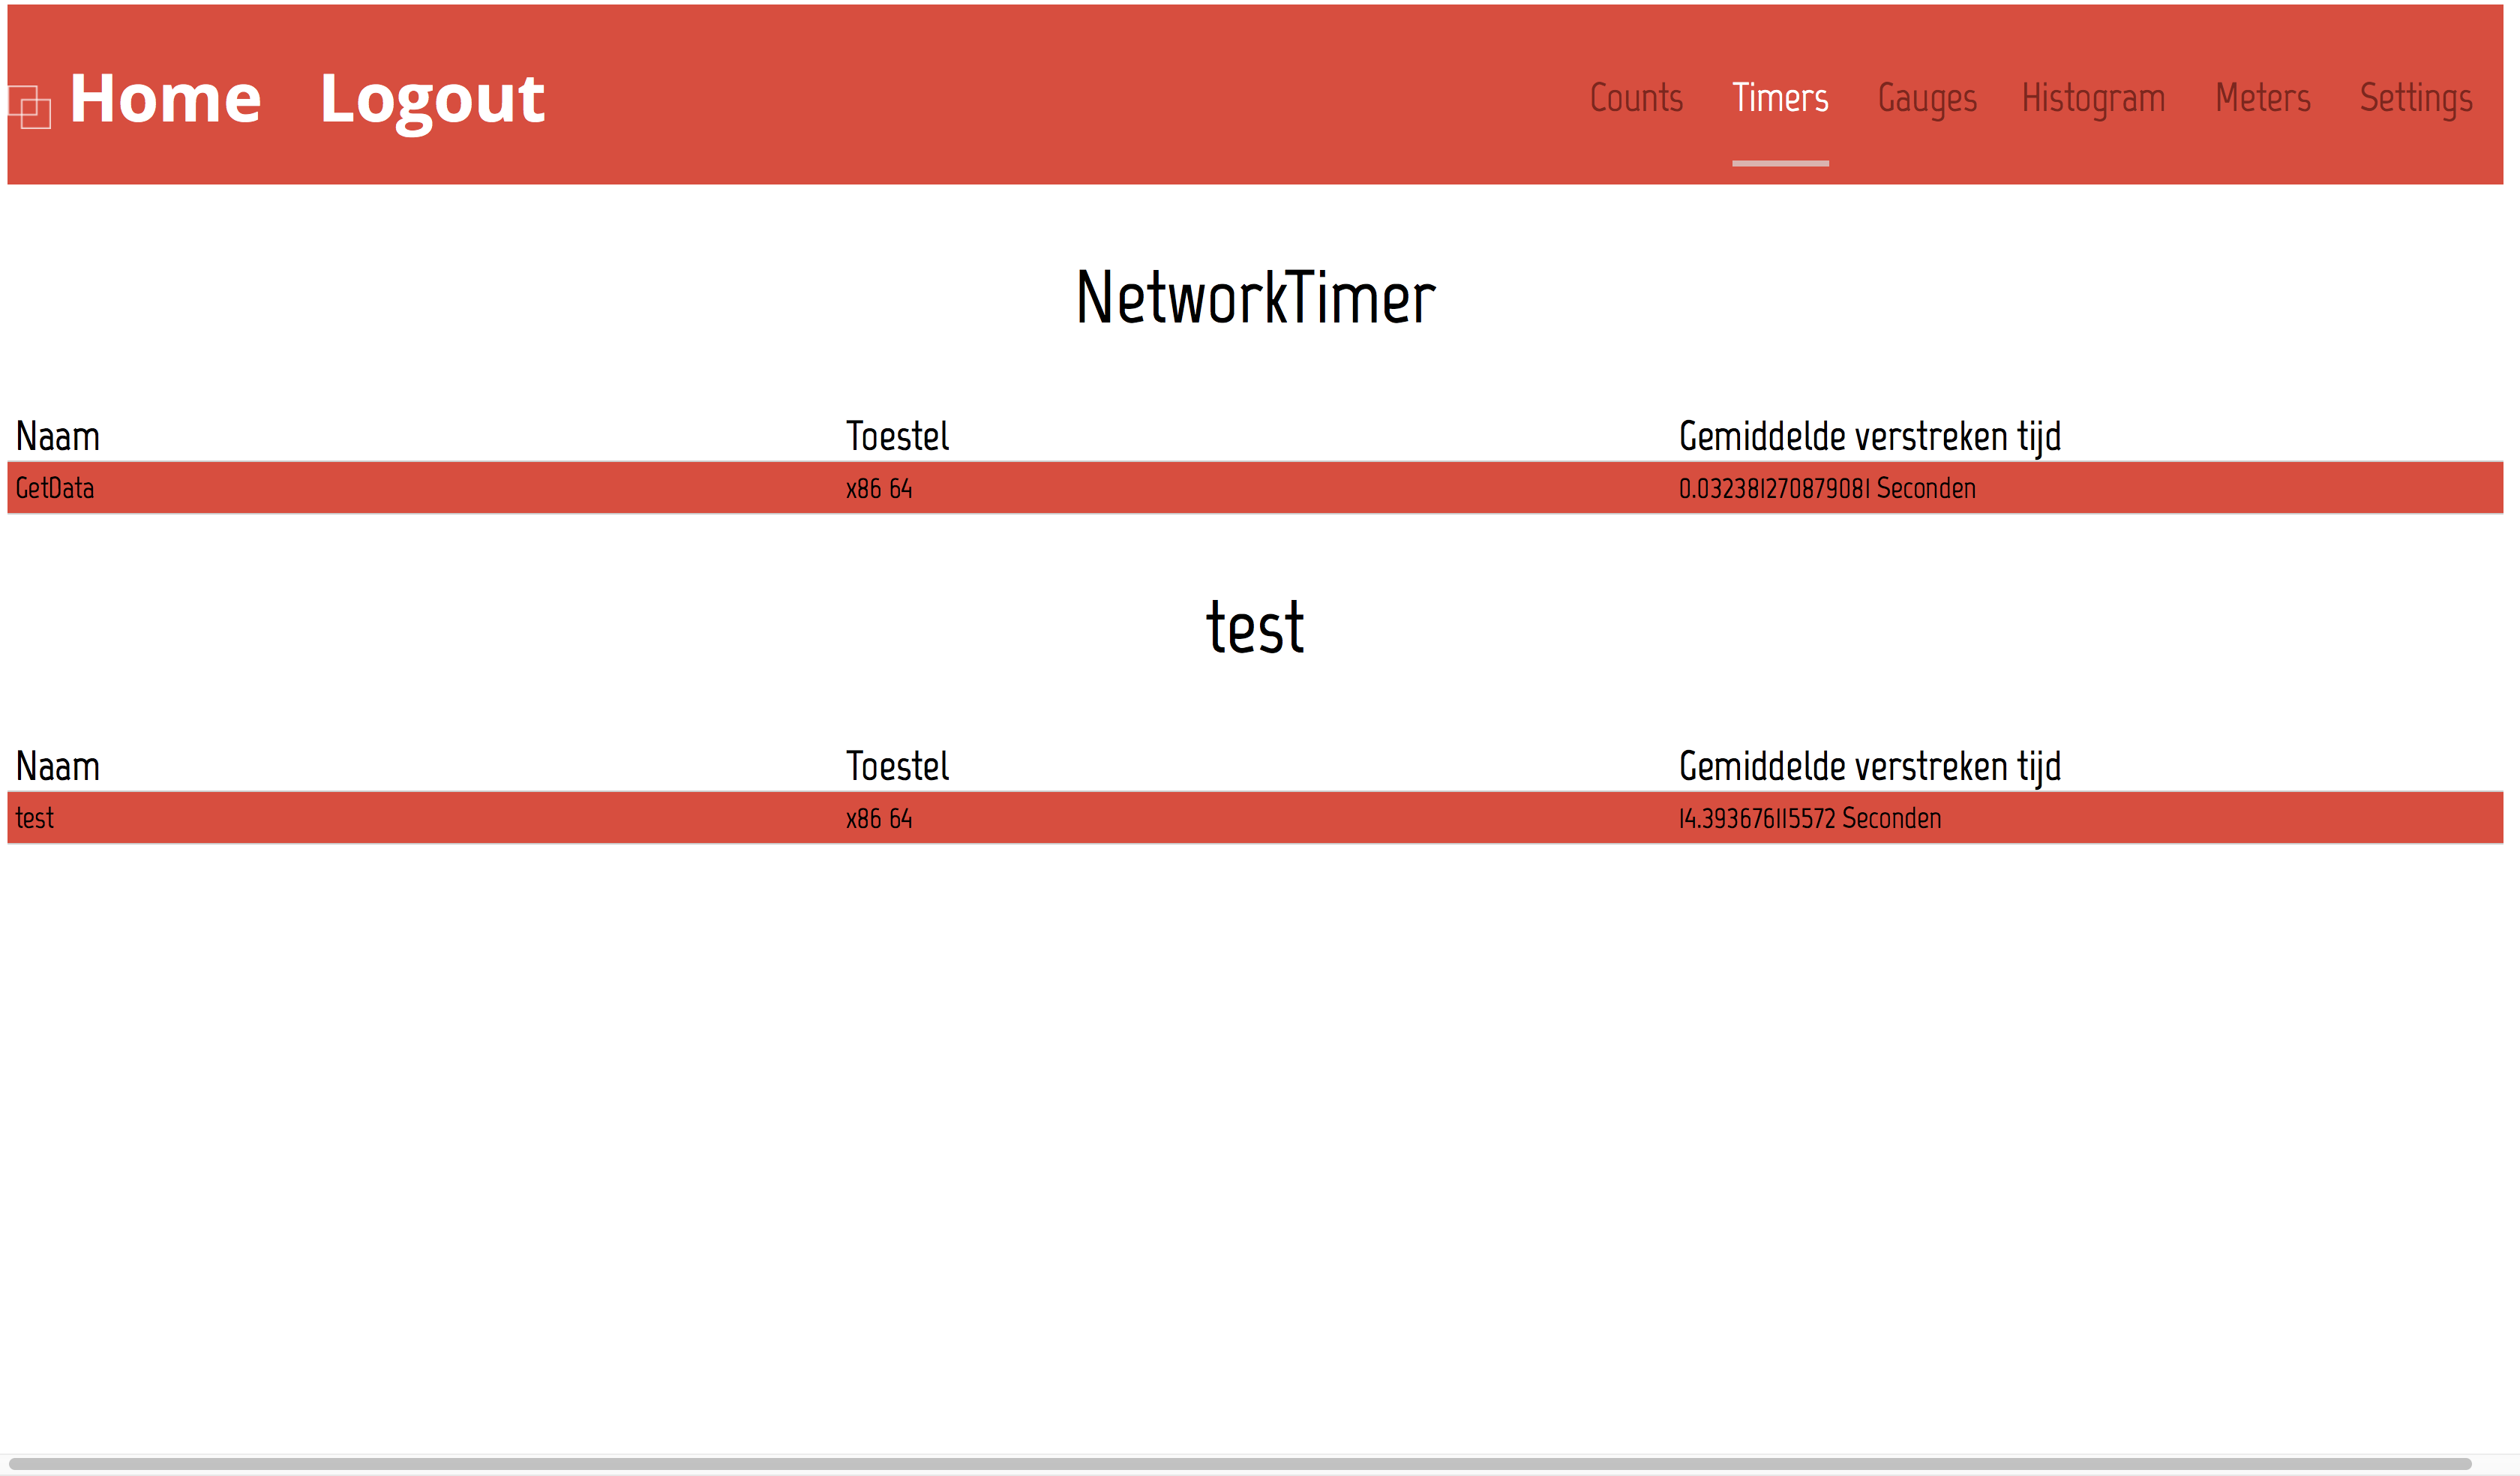
\includegraphics[scale=0.2]{Afbeeldingen/Implementatie/Timer}
  \caption{Dashboard: \texttt{Timer} overzicht.}
  \label{fig:DasbhoardTimer}
\end{figure}

\begin{figure}[!h]
  \centering
  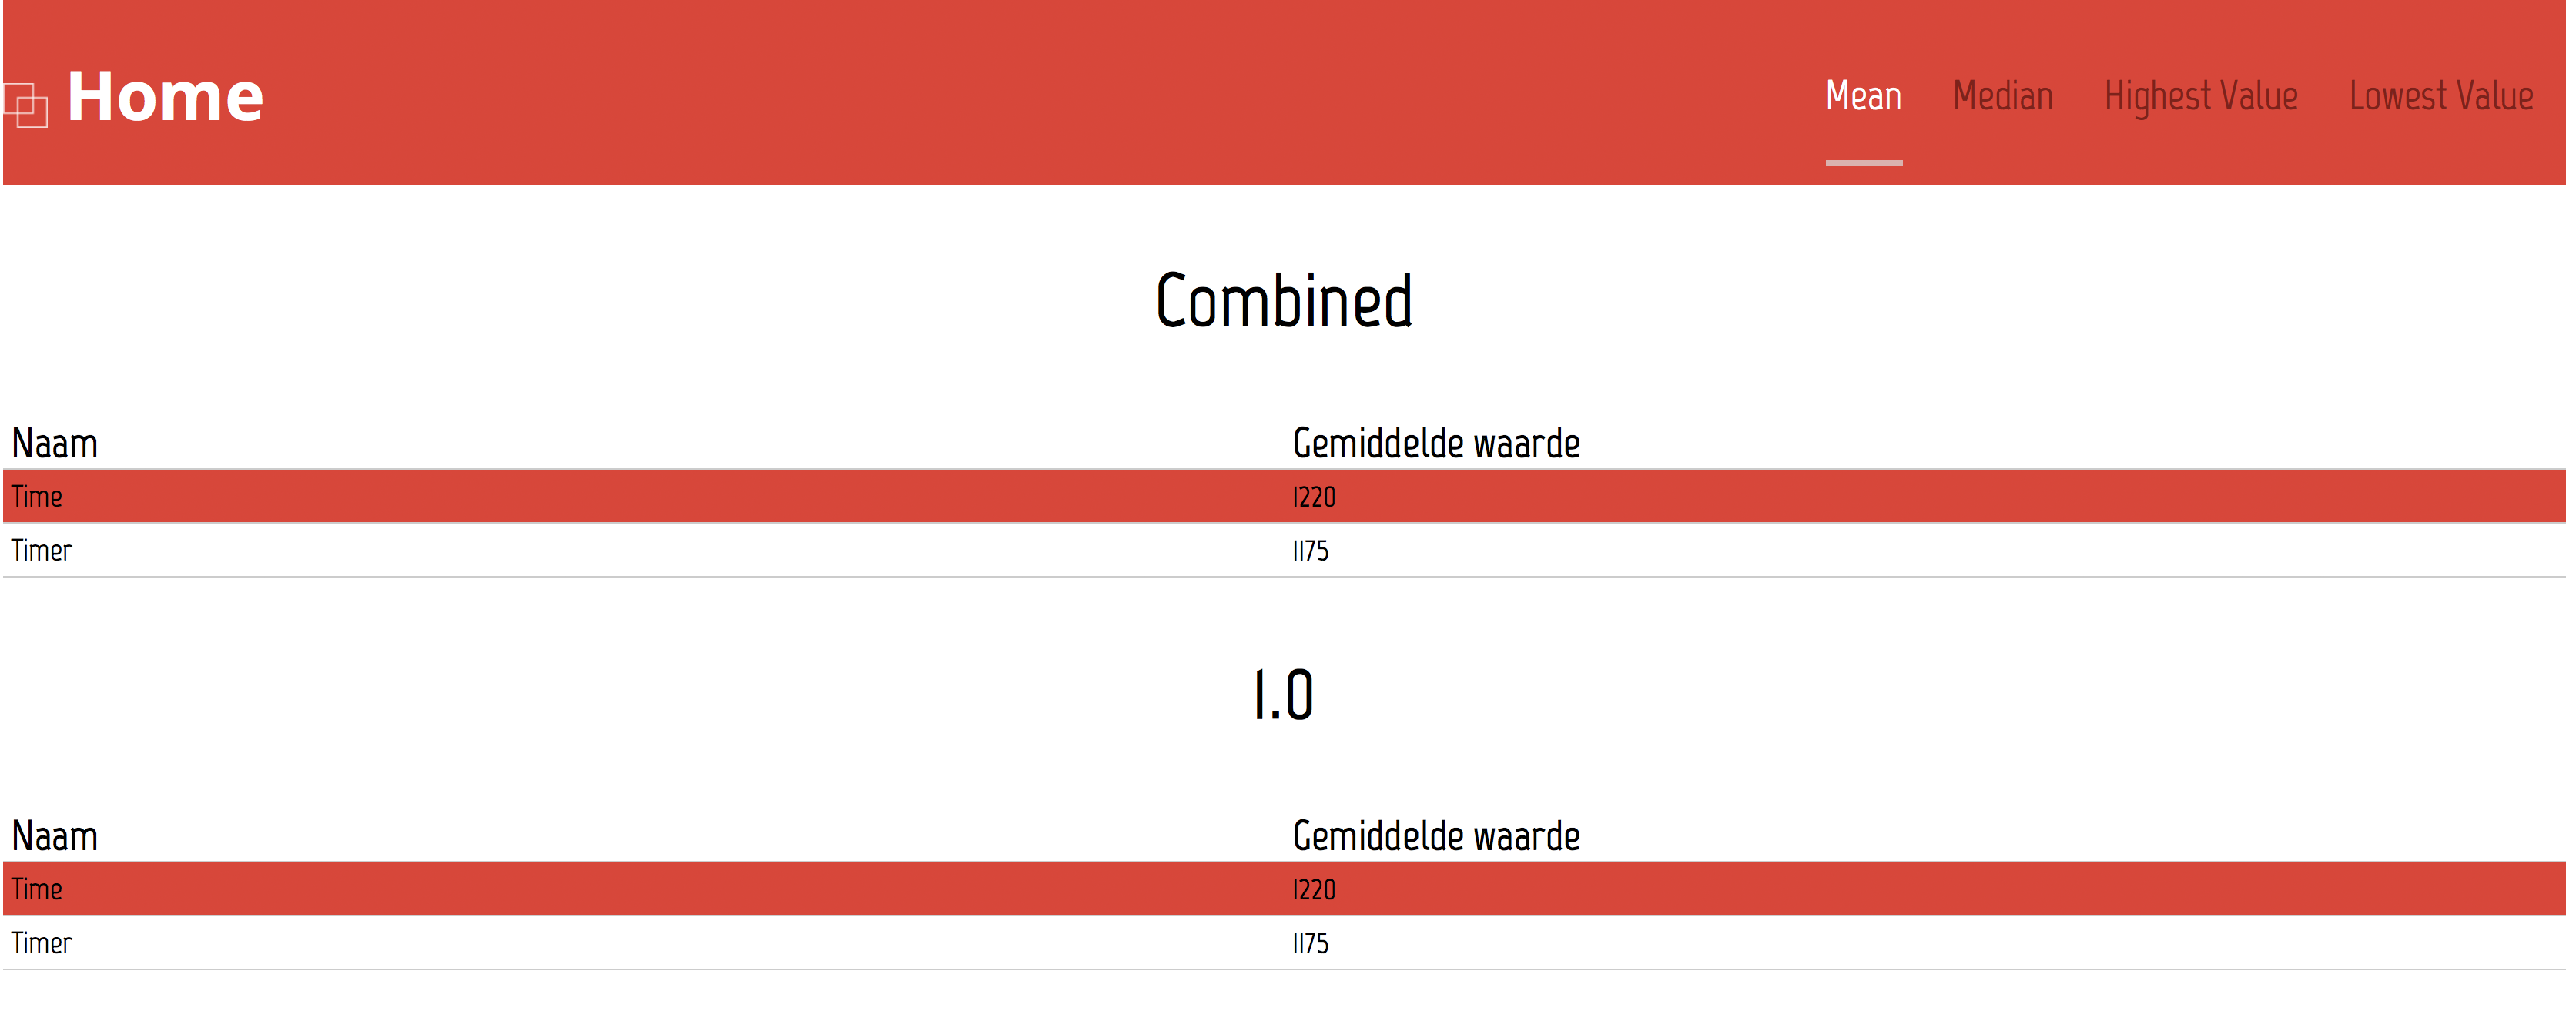
\includegraphics[scale=0.2]{Afbeeldingen/Implementatie/Timer-Combined}
  \caption{Dashboard: \texttt{Timer} overzicht per versie.}
  \label{fig:DasbhoardTimerCombined}
\end{figure}

\begin{figure}[!h]
  \centering
  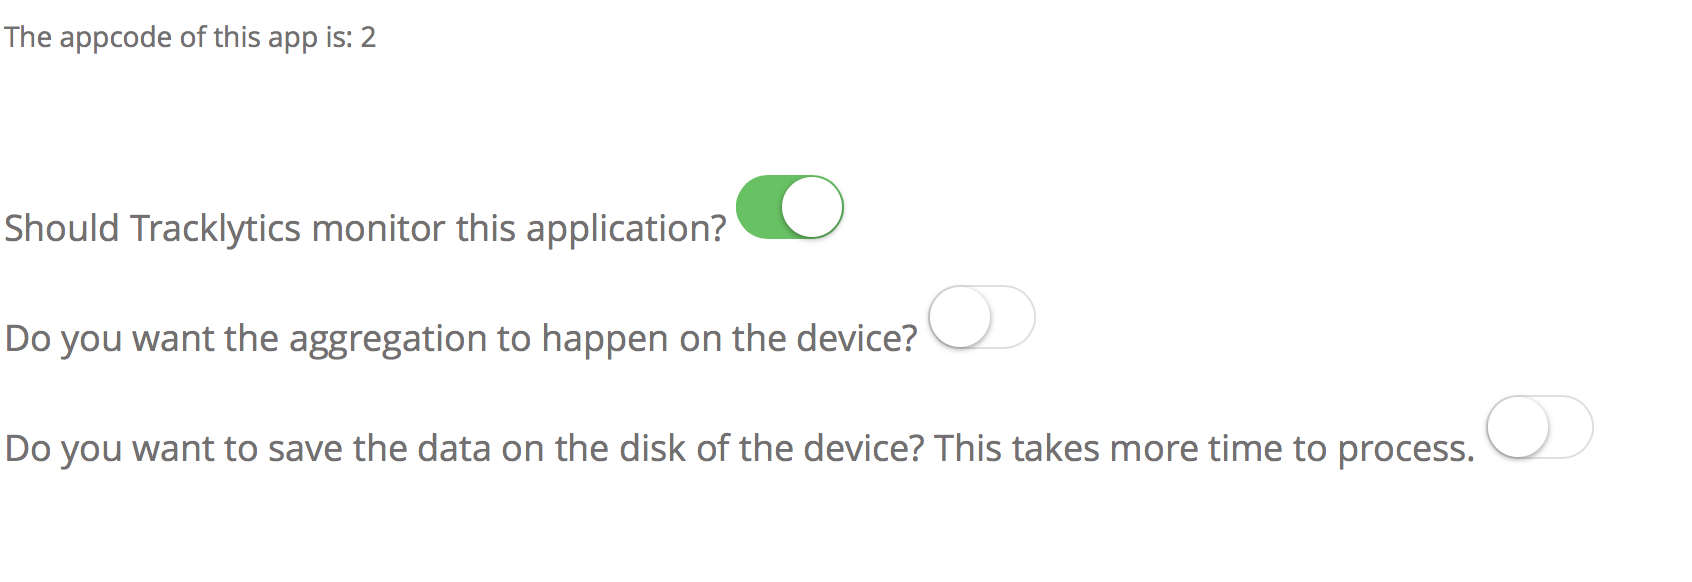
\includegraphics[scale=0.2]{Afbeeldingen/Implementatie/Settings}
  \caption{Dashboard: Instellingen overzicht.}
  \label{fig:DasbhoardSettings}
\end{figure}







\subsection{Connectie tussen Front end en Back end}
Zoals eerder aangegeven stuurt de front end (de Tracklytics iOS library) data naar de back end over een internetverbinding. Om ervoor te zorgen dat deze data veilig overgedragen wordt, werd ervoor gekozen om een HTTPS verbinding te gebruiken. Dit zorgt er automatisch voor dat er een veilige verbinding tussen client en server bestaat. Een alternatief is de data zelf encoderen aan de client zijde en decoderen aan de server zijde. Omdat HTTPS ervoor zorgt dat de data veilig wordt overgedragen werd ervoor gekozen om encoderen en decoderen niet te gebruiken.
Een andere beveligingskeuze die er gemaakt werd om HTTP POST te gebruiken in plaats van HTTP GET. HTTP POST verbergt de data in de request, terwijl HTTP GET de data in de URL van de request zet. De consequenties hiervan zijn dat de data in HTTP POST requests in geen enkele log of geschiedenis voorkomen, wat wel kan gebeuren met HTTP GET requests. Het is ook moeilijker de data in de HTTP POST requests aan te passen dan die van de HTTP GET requests, omdat het gemakkelijker is om een URL aan te passen dan een request zelf.\\

\section{Aggregatie}
De data die de Tracklytics library opgehaald heeft bij het monitoren van de applicatie moet geaggregeerd worden om weer te kunnen geven in het dashboard. De logische plaats om deze aggregatie uit te voeren is de back end, omdat deze elk meetpunt in de database heeft staan. Het voordeel hieraan is dat de data opgehaald kan worden en enkel verwerkt wordt wanneer deze nodig is. Een nadeel hieraan is dat dit zeer veel CPU kan kosten en zo het dashboard enorm traag maakt. Dit nadeel is gelinkt aan de hoeveelheid gebruikers van de applicatie en het aantal meetpunten in de applicatie. Groeit een van beide of beiden, dan treedt er een extra vertraging op in het aggregeren van de gegevens. Dit probleem kan opgelost worden door op voorhand te aggregeren, dit kan op twee manieren: \textbf{op het toestel zelf} en \textbf{op periodieke intervallen}. Deze sectie berust zich op het feit dat I/O operaties veel trager zijn dan verwerkingsoperaties.\\

De eerste oplossing is om de aggregatie uit te voeren op het toestel zelf. De Tracklytics library kan aangepast worden om in plaats van de data van de meetpunten zelf door te sturen, eerst deze te verwerken op het toestel zelf en die verwerkte data door te sturen naar de server. De back end zal ook moeten aangepast worden om deze data op te slaan zodat deze herbruikt kan worden. Het voordeel hieraan is dat als het dashboard de data opvraagt van de back end, de back end dit sneller zal kunnen doen, omdat er minder data uit de database opgehaald en verwerkt moet worden. Zo wordt het dashboard bruikbaarder bij grotere schaal. Een nadeel hieraan is dat de gegevens niet meer optimaal zijn. Bijvoorbeeld: de mediaan kan enkel nog benaderd worden, omdat niet alle waarden aanwezig zijn in de database. Door afrondingsfouten kunnen de gemiddeldes verschillen van de werkelijke gemiddeldes. \\

Een tweede oplossing is om periodiek (bv. \'e\'en keer per dag) per applicatie de nieuwe data te gaan aggregeren en samenvoegen met de al geaggregeerde data van de voorbije tijdstippen. Deze functionaliteit moet op de servers ge\"implementeerd worden. Het voordeel hieraan is dat indien het dashboard de data opvraagt, enkel de nieuwe data nog moet samengevoegd worden met de al geaggregeerde data. Dit zorgt voor een enorme performance boost van het dashboard. Het nadeel hieraan is dat ofwel er een overzicht moet bijgehouden worden welke data al geaggregeerd is en welke niet, ofwel de verwerkte data telkens uit de database verwijderd moet worden om delen van de dataset niet opnieuw te verwerken. Dit vraagt dus een extra inspanning om te implementeren. \\

Een derde oplossing is om de twee te combineren. Op het toestel wordt een deel van de aggregatie al gedaan en deze geaggregeerde data wordt dan verwerkt op de servers zoals in het vorige deel. Dit geeft een extra prestatiewinst, de verwerking van de geaggregeerde data op de servers gaat sneller, omdat deze al geaggregeerd werd. Er is dus minder CPU-tijd nodig om de opdracht af te werken. Indien het dashboard de data opvraagt aan de back end gaat dit ook veel sneller. De combinatie van de nieuwe data en geaggregeerde data gaat veel sneller, omdat er minder data aanwezig is. \\

Een laatste oplossing is om de data te aggregeren wanneer het echt nodig is en deze dan op te slaan. Als de developer of eigenaar van de applicatie het dashboard voor de eerste keer opent, dan wordt deze data geaggregeerd en opgeslagen zoals bij de tweede oplossing. Als de developer of eigenaar het dashboard de volgende keer opent moet enkel de nieuwe data geaggregeerd worden en gecombineerd met de al geaggregeerde data. Deze combinatie wordt dan opnieuw opgeslagen. Dit proces wordt herhaald telkens dat het dashboard van die applicatie geopend wordt. Het voordeel hieraan is dat dit sneller is dan telkens opnieuw alle data te aggregeren. Het nadeel hieraan is dat er moet bijgehouden worden welke data verwerkt is en welke niet. \\


In de Tracklytics library werd ervoor gekozen om de developer de keuze aan te bieden tussen het aggregeren van de data in de back end en het aggregeren van de data op het toestel. De Tracklytics library aggregeert data van de volgende meetobjecten op het toestel: \textbf{Gauge, Meter, Timer}. De developer kan deze keuze maken in de instellingen die het dashboard aanbiedt. \\

\paragraph{Het Gauge meetobject} wordt geaggregeerd op het toestel door tijdens het aggregeren \textit{het gemiddelde, de mediaan, de laagste en de hoogste waarde} te berekenen op basis van de waarden die gemeten worden. In plaats van telkens een nieuwe Gauge waarde aan te maken, wordt deze toegevoegd aan een helper object die deze waarden bijhoudt om de mediaan te berekenen en bij het toevoegen van een waarde ineens het gemiddelde berekent en bekijkt of deze waarde de hoogste of laagste waarde is. Het grootste nadeel hieraan is dat de mediaan in de back end enkel nog benaderd kan worden omdat niet alle waarden nog in de back end aanwezig zijn. \\

\paragraph{Het Meter meetobject} wordt als volgt geaggregeerd: in plaats van elke waarde apart op te slaan wordt het aantal metingen bijgehouden en wordt er een gemiddelde bij gehouden. Deze waardes kunnen in de back end gecombineerd worden om een globaal overzicht te krijgen. Het nadeel hieraan is dat er afrondingsfouten kunnen gebeuren bij het berekenen van het gemiddelde en er zo een verkeerde observatie gemaakt kan worden. Ook wordt er niet per meting bijgehouden op welk tijdstip deze voorvalt. \\

\paragraph{Het Timer meetobject} wordt geaggregeerd door de gemiddelde tijd te berekenen bij het stoppen van een timer en bij te houden hoeveel metingen er voorgekomen zijn. Het nadeel is dat er per timer maar \'e\'en instantie tegelijkertijd kan lopen omdat Tracklytics dezelfde methodes aanbiedt voor een geaggregeerd object en een niet-geaggregeerd object. Net zoals bij het \textit{Meter meetobject} kunnen er hier afrondingsfouten voorkomen. \\



\section{Openstaande uitdagingen}
De implementatie gegeven in deze thesis dekt niet de volledige architectuur uit de vorige sectie. Er blijven dus nog steeds uitdagingen om de library uit te breiden zodat deze dichter aanleunt bij de architectuur. Er worden ook andere uitbreidingen beschreven die niet in de architectuur beschreven worden, maar van even groot belang zijn dan degene die wel in de architectuur beschreven wordt. 

\subsection{AB Testing}
AB testing wordt gebruikt om geleidelijk aan een nieuwe versie van een applicatie of website uit te rollen, zoals beschreven in de architectuur sectie. Het vormt een uitdaging om dit concept te combineren met de Tracklytics library. Er moet onderzocht worden wat de effici\"entste manier is om AB testing in mobiele applicaties mogelijk te maken.  Een manier om AB testing te gebruiken is om eerst het versienummer voor die gebruiker op te halen in de database. Een niet effici\"ente manier zou dan zijn om per versie een if statement te gebruiken om zo de verschillende karakteristieken van de versie te bepalen. Deze manier is op drie manieren ineffici\"ent, namelijk: de code van de applicatie (en dus ook de grootte op schijf) wordt groter naarmate er meer versies worden gebruikt, door de if statements wordt de applicatie trager en als er een aanpassing moet gebeuren aan een versie of er wordt een versie toegevoegd moet deze nog steeds eerst via de app store als update uitgevoerd worden.


\subsection{Operating systems} 
De Tracklytics library werd ontwikkeld voor iOS, het besturingssysteem van Apple. Er bestaat buiten iOS nog een besturingssysteem dat de moeite waard is om te bekijken, namelijk Android. Op het moment van schrijven is Android de marktleider met een marktaandeel van 59.65\% in de mobiele markt, gevolgd door iOS (32.28\%) \cite{MarketShare}. De andere mobiele besturingssystemen zijn niet de moeite waard om te bekijken, omdat deze een bijna verwaarloosbaar marktaandeel hebben. De toestellen die Android gebruiken zijn verdeeld over vele versies. Op moment van schrijven draait ongeveer een derde van de toestellen op een twee jaar oud besturingssysteem (KitKat 4.4) \cite{AndroidMS}. In contrast, 84\% van de toestellen die op iOS draaien hebben de laatste versie ge\"installeerd (op moment van schrijven) \cite{iOSMS}. Elke nieuwe versie brengt veranderingen en vernieuwingen met zich mee, wat er voor zorgt dat sommige taken sneller/trager uitgevoerd worden in de ene versie dan in de andere versie. Dit heeft mede de keuze voor iOS gemaakt. \\

De uitdaging die zich hier voordoet is het schrijven van een library voor Android. Dezelfde architectuur kan worden gebruikt voor de library. Er moeten enkele aanpassingen gedaan worden om dit te doen werken. Allereerst moet er een onderscheid gemaakt kunnen worden tussen iOS en Android data. Door telkens het type besturingssysteem door te sturen als metadata wordt dit mogelijk om het zo in de database te stoppen. Anderzijds is het noodzakelijk in het Android geval om de versie van het besturingssysteem mee door te sturen, zodat er in het dashboard een duidelijke opdeling kan gemaakt worden. Dit zorgt er dan weer voor dat het dashboard complexer wordt om te implementeren.





\subsection{Alarmen}
%alarmen als bepaalde waarde over iets gaat of als gemiddelde timer hoger wordt dan ...
Om het concept en nut van alarmen uit te leggen is het handig om met een voorbeeld te beginnen. 

Een eigenaar heeft een applicatie ontwikkeld die communiceert met de back end. De eigenaar heeft ervoor gekozen om servers te huren in plaats van zijn eigen servers te bouwen en onderhouden. De eigenaar wil dat er zo weinig mogelijk servers gehuurd moeten worden en dat de gebruiker van de applicatie geen zichtbare vertraging heeft (er toch genoeg servers zijn om de requests te behandelen). Zo kunnen de kosten geminimaliseerd worden en dus de winst gemaximaliseerd. Developers moeten dus servers toevoegen als de servers de requests niet meer aan kunnen en een server verwijderen indien die server overbodig wordt om het werk gedaan te krijgen. 

Om dit mogelijk te maken moet er een trigger of alarm komen die de developers waarschuwt indien de huidige servers het werk niet meer snel genoeg kunnen doen. Dit alarm kan ge\"implementeerd worden in de servers of in de Tracklytics library. \\

Er bestaan al meerdere oplossingen die deze functionaliteit aanbieden op het vlak van servers. Hier wordt niet verder op ingekeken omdat dit niet in de context van deze thesis past. \\

In de Tracklytics library kan er een alarm functionaliteit aangeboden worden. Een developer moet dan in het dashboard aangeven welke parameter welke waarde maximum mag krijgen. Het is ook handig dat de developer een maximum aantal schendingen van deze parameter kan aangeven en dat hij enkele types van metadata kan uitsluiten. (bv. de tijd dat het kost om data van de back end op te halen mag maximum bij 5 verschillende gebruikers boven de 10 seconden liggen op WiFi en 4G). De developer moet ook de tijdspanne aanduiden waarin deze parameters niet overschreden mogen worden. Indien deze drempel overschreden wordt, moet er een waarschuwing gestuurd worden naar de developer. Hierdoor moeten de drie componenten samenwerken (Dashboard, Back end en mobiele library). Het dashboard moet de gegeven parameters doorgeven aan de back end zodat deze opgeslagen kunnen worden in de database. De mobiele library moet, via de back end, de parameters ophalen. Indien er zich dan een match voordoet wanneer er nieuwe gegevens worden doorgegeven via de applicatie, dan moet de library nagaan of deze de drempel niet overschrijden. Indien de drempel wordt overschreden, dan moet dit gemeld worden aan de back end. De Tracklytics library moet dan een call doen naar de back end. De back end slaat deze melding op in de database en gaat na of er een alarm verstuurd moet worden. De back end kijkt dus of er in de gegeven tijdspanne meer schendingen geweest zijn dan dat de developer als maximum aangaf. In plaats van elke keer dat er een schending is na te gaan of er een alarm verstuurd moet worden, kan de back end periodiek nagaan of de parameters overschreden worden. Het voordeel hieraan is dat de back end sneller is, omdat de controle niet telkens moet uitgevoerd worden. Het nadeel is dat het alarm bijna een volledige periode later uitgezonden wordt indien de schending van de parameters aan het begin van de periode plaatsvindt. \\

De alarm functionaliteit kan ervoor zorgen dat er zo weinig mogelijk servers gebruikt worden en het geen impact heeft op de kwaliteit van de applicatie en niet zichtbaar is voor de gebruikers. Zo kunnen de kosten geminimaliseerd worden en de winst gemaximaliseerd. 